\documentclass[12pt, a4paper]{ctexart}

\usepackage{amsmath}
\usepackage{amssymb}
\usepackage{amsthm}
\usepackage{geometry}
\usepackage{graphicx}
\usepackage{booktabs}
\usepackage{bm}
\usepackage{hyperref}
\usepackage{algorithm}
\usepackage{algpseudocode}
\usepackage{cite}
\usepackage{caption}

\geometry{left=2.5cm, right=2.5cm, top=3.0cm, bottom=3.0cm}

\theoremstyle{plain}
\newtheorem{assumption}{假设}
\newtheorem{definition}{定义}
\newtheorem{lemma}{引理}
\newtheorem{proposition}{命题}
\newtheorem{theorem}{定理}
\newtheorem{corollary}{推论}
\theoremstyle{remark}
\newtheorem{remark}{注记}

\title{\textbf{基于形状感知体积符号距离场与半光滑牛顿法的\\高精度接触动力学框架}}
\author{匿名作者}
\date{\today}

\begin{document}

\maketitle

\begin{abstract}
针对传统多体动力学（MBD）中点接触法线跳变、罚函数模型的刚度-步长耦合，以及有限接触斑扭转载荷难以进入统一接触律等问题，本文建立了一套基于隐式符号距离场（SDF）的接触动力学理论框架。本文的核心并非单独提出一种新的互补求解器，而是构造一条从分布式重叠几何到有限维接触律的理论闭环。具体而言，本文首先以局部重叠深度场的矩比泛函定义量纲一致的形状感知等效间隙，并证明其具备有界性、关于形状敏感指数$p$的单调聚焦性质、对尖锐特征的高阶矩放大能力，以及在小穿透极限下与经典法向间隙的一致性。随后，本文在同一权函数测度下统一定义等效接触中心、等效法线、扭转惯性半径与切向-扭转雅可比，得到由分布式接触斑向有限维接触结构的几何压缩映射，并证明其在叠加刚体运动下的协变性。进一步地，本文给出带退化正则化的四维摩擦锥，证明其在有限接触斑上能够表达抗扭转载荷，并在接触斑塌缩时连续退化为经典三维库仑摩擦。最后，在上述几何与力学结构基础上，本文将离散接触动力学写成二阶锥互补问题（SOCCP），并采用Jordan代数与Fischer-Burmeister函数建立半光滑牛顿求解框架。该框架为后续实现复杂刚柔耦合系统中的非光滑接触计算提供了统一的几何、力学与算法基础。对于当前均匀体素原型，本文仅对$p=2\sim4$给出数值层面的工程性主张，而将$p=6$保留为展示高阶聚焦趋势的理论示例；要使更高$p$成为稳健默认配置，仍需自适应积分支持。本文当前的数值证据仍以解析刚体SDF原型为主，但已额外包含一个受控扭转载荷解析参照、一个耦合平动-扭转状态下的独立4D PGS交叉验证、一个非轴对称3D torsion-free场景中的独立polyhedral friction外部基线，以及一个两接触盒体堆叠中的解析/闭合三角网格mesh-SDF对照，并统一报告raw residual、scaled residual与锥互补违约，从而分别补强四维摩擦主链的正确性证据、torsion-free friction主链的外部交叉验证、求解器独立交叉验证和几何外延性证据。

\textbf{关键词：} 多体系统动力学；符号距离场（SDF）；矩比等效间隙；四维库仑摩擦；二阶锥互补问题（SOCCP）；半光滑牛顿法
\end{abstract}

\newpage
\tableofcontents
\newpage

\section{引言 (Introduction)}
\subsection{研究背景与动机}
接触与摩擦是多体系统动力学（Multibody System Dynamics, MBD）以及刚柔耦合系统中最具挑战性的非光滑物理过程之一。困难并不只在于“是否检测到接触”，而在于如何把连续分布的几何重叠、法向压缩与切向滑移压缩成一个既满足物理客观性、又便于离散求解的有限维接触律。传统工业软件与物理引擎大多依赖离散表面网格（Polygonal Meshes）和局部点接触描述：几何层面上，它们以接触点和法线为基本变量；动力学层面上，它们再在这些局部量上施加罚函数、冲量或互补约束。这一路线虽然工程上高效，但在接触点切换、接触斑生成与消失、尖锐特征进入或退出接触时，常常出现法线演化不连续与随之而来的接触抖动，继而在时域积分中诱发非物理高频震荡\cite{lu2011isogeometric,noels2006crashworthiness}。

若进一步考虑有限接触斑而非理想点接触，问题会更加复杂。真实接触中，法向反力并非集中于一点，切向耗散也往往伴随由接触斑尺度诱导的扭转载荷；然而传统点接触模型通常只保留法向间隙和二维切向滑移，因而难以在统一框架下解释“几何分布如何进入有限维摩擦律”。从理论上说，这一缺口体现在三个彼此耦合的问题：其一，如何定义一个对尖锐几何特征足够敏感、同时又具有明确量纲和经典极限的一维等效法向间隙；其二，如何把面接触或体积接触所诱导的分布式切向滑移与扭转载荷压缩为有限维摩擦结构；其三，如何在保留前两者几何来源的前提下，将接触条件转化为适于大规模数值求解的互补系统。

本文的出发点正是同时回应这三个问题。我们并不把“求解器本身”作为唯一创新目标，而是试图建立一条从\emph{局部重叠深度场}出发、经过\emph{等效间隙和等效接触几何}、最终落到\emph{有限维摩擦律与SOCCP表述}的完整理论链条。只有当这条链条在量纲、一致性、退化极限与客观性上都闭合时，后续数值算法才真正具备可解释性。

\subsection{相关工作与本文定位}
现有工作大致可归为三条路线。第一条是\textbf{点接触/罚函数路线}。其优势在于实现简单、易于嵌入现有求解器，但接触刚度与时间步长之间存在显著耦合：刚度过小会产生较大穿透，刚度过大则引发强刚性，使显式或弱隐式时间推进高度敏感\cite{hunek1993penalty,kolman2021bipenalty}。更关键的是，这一路线默认接触可以由少数局部点代表，因此当接触实际以有限接触斑形式出现时，扭转载荷往往只能通过经验修正进入模型，而缺乏直接的几何来源。

第二条是\textbf{隐式几何与体积积分路线}。SDF为任意空间点提供连续的穿透信息与梯度，天然适合用于缓和B-Rep离散法线带来的切换不连续性；体积积分或欧拉式接触思想则进一步把注意力从“接触点”转向“接触区域”。这一方向在几何平滑性上明显优于传统点接触，但代表性工作更多把积分量作为接触区域上的惩罚型、体积型或相场型约束来使用，因此其量纲解释、点接触极限以及有限接触斑扭转载荷的统一有限维表达，并非既有理论的主要目标\cite{leichner2019implicit,lorez2024eulerian}。

第三条是\textbf{互补问题、变分不等式与非光滑求解路线}。该方向已经为法向不可穿透、库仑摩擦以及半光滑牛顿型算法提供了坚实的离散理论与数值分析工具。然而在大多数工作中，接触法线、接触点或接触斑参数往往被当作先验输入，求解器负责处理“给定变量上的互补结构”，却较少回答这些变量本身如何由连续接触几何严格诱导。

基于上述观察，本文的定位并不是再提出一种孤立的SOCCP算法变体，而是补上几何与求解之间长期缺失的一环：从\textbf{局部重叠深度场}出发，经由\textbf{量纲一致的等效间隙}和\textbf{统一测度下的接触几何压缩映射}，构造出可退化到经典点接触理论的\textbf{有限维摩擦律}，再在此基础上引入SOCCP与半光滑牛顿法。换言之，本文强调的主创新是\emph{几何诱导的有限维接触律理论}，而不是把成熟的互补求解技术本身重新包装为唯一贡献。

\subsection{理论缺口与本文主线}
综合上述文献可以看出，当前最缺少的并不是某一种局部数值技巧，而是一套同时满足以下要求的接触理论：\textbf{(i) 等效法向量纲明确并可解释为运动学间隙；(ii) 对尖锐重叠具有可证明的敏感性，而不是仅靠经验参数调节；(iii) 在接触斑塌缩时能连续退化到经典点接触理论；(iv) 能自然诱导扭转载荷并与有限维互补结构兼容}。如果这四点不能同时满足，那么要么几何量缺乏明确物理解释，要么有限维摩擦律与原始分布式接触之间脱节，要么点接触极限与已有理论不一致。

本文以“局部重叠深度的矩比等效间隙”为主轴来组织上述问题。第一步，我们不直接把体积积分或未归一化$L_p$量当作间隙，而是构造量纲正确的矩比泛函，借此得到既可调聚焦又具有经典极限的一维法向量。第二步，我们在同一权函数测度下定义接触中心、法线、扭转尺度和切向雅可比，从而保证所有有限维接触变量来自同一几何压缩原则。第三步，我们在这一压缩映射基础上建立带退化正则化的四维摩擦锥，并证明它对有限接触斑有效、对点接触极限一致。最后，SOCCP与半光滑牛顿法只承担“把上述理论结构离散化并求解”的角色，从而形成清晰的理论层次。

\subsection{本文的主要贡献}
为解决上述挑战，本文提出了一套完备的基于积分的接触动力学与数值求解框架，主要贡献如下：
\begin{enumerate}
    \item 提出一种\textbf{量纲一致的形状感知等效间隙泛函}。不同于直接采用体积积分或未归一化$L_p$范数，本文以局部重叠深度场的\textbf{矩比泛函}定义全局等效间隙，使其保持长度量纲、对深穿透区域具有可调聚焦能力，并在理论上满足单调性、上界一致性与$p \to \infty$极限性质。
    \item 提出一种\textbf{由重叠深度诱导的接触几何压缩映射}。通过统一的权函数测度，同时定义等效接触中心、等效法线、扭转惯性半径与等效切向雅可比，从而将分布式体积接触压缩为有限维接触结构，并证明其在刚体运动下的协变性与点接触极限下的退化一致性。
    \item 构建一套\textbf{从分布式摩擦耗散到四维有限维摩擦律}的理论链条。本文给出切向滑移映射的一阶精确性分解，并引入带退化正则化的四维摩擦锥，使模型在面接触时能够表达抗扭转载荷，在接触斑塌缩为点时又能连续退化为经典三维库仑摩擦。
    \item 在上述几何与接触律基础上，将问题进一步表述为SOCCP，并采用Jordan代数与Fischer-Burmeister函数构造半光滑牛顿求解框架。本文将该部分定位为\textbf{理论闭环与数值实现手段}，而非全文唯一创新来源。
\end{enumerate}

\begin{table}[htbp]
    \centering
    \caption{本文创新边界的定位图（novelty map）}
    \label{tab:novelty_map}
    \footnotesize
    \setlength{\tabcolsep}{4pt}
    \renewcommand{\arraystretch}{1.15}
    \begin{tabular}{p{1.9cm}p{3.9cm}p{5.0cm}p{3.7cm}}
        \toprule
        层次 & 既有工作中常见做法 & 本文的新增内容与定位 & 本文不主张的新意 \\
        \midrule
        几何层 & 点接触法向间隙、体积罚项或未归一化积分量 & 以矩比泛函$-I_p/I_{p-1}$定义量纲一致的等效间隙，并在同一测度下统一压缩$\bm{p}_c,\bm{n}_c,r_\tau,\bm{J}_t$ & SDF本身、体素积分本身并非本文新意 \\
        摩擦层 & 经典三维库仑锥，或以经验项附加扭转载荷 & 从有限接触斑的一阶滑移压缩出带扭转分量的四维摩擦结构，并证明其在接触斑塌缩时连续退化到经典三维库仑摩擦 & 库仑摩擦定律本身并非本文提出 \\
        求解层 & 互补问题、SOCCP、Fischer--Burmeister函数与半光滑牛顿等非光滑求解技术 & 将SOCCP/FB/SSN作为保持上述几何与摩擦结构的离散实现手段，而非把求解器本身包装成唯一创新点 & SOCCP或半光滑牛顿作为独立算法并非本文主要贡献 \\
        \bottomrule
    \end{tabular}
\end{table}

\section{符号体系、局部重叠深度与基本假设}
\subsection{符号约定}
设刚体或柔性体$A$与$B$由各自的符号距离场（SDF）$\phi_A(\bm{x};\bm{q})$与$\phi_B(\bm{x};\bm{q})$隐式表示，其中$\bm{q}$为系统广义坐标。记正部算子为$(a)_+ = \max(a,0)$。本文定义两个局部穿透深度场
\begin{equation}
    \delta_A(\bm{x};\bm{q}) = (-\phi_A(\bm{x};\bm{q}))_+, \qquad
    \delta_B(\bm{x};\bm{q}) = (-\phi_B(\bm{x};\bm{q}))_+ .
\end{equation}
对应的重叠域记为
\begin{equation}
    \Omega(\bm{q}) = \{ \bm{x} \in \mathbb{R}^3 \mid \delta_A(\bm{x};\bm{q}) > 0,\; \delta_B(\bm{x};\bm{q}) > 0 \} .
\end{equation}

\begin{definition}[局部重叠深度聚合器]
为保持长度量纲并与后续半光滑分析兼容，本文采用
\begin{equation}
    \delta(\bm{x};\bm{q}) = \min\{ \delta_A(\bm{x};\bm{q}), \delta_B(\bm{x};\bm{q}) \}
\end{equation}
作为局部重叠深度。更一般地，也可将$\delta$推广为满足\textbf{对称性、一阶齐次性、Lipschitz连续性}的聚合器$\Psi(\delta_A,\delta_B)$；本文将上述$\min$定义作为基准模型。
\end{definition}

\subsection{基本假设}
\begin{assumption}[SDF正则性]\label{ass:sdf}
在感兴趣的接触邻域内，$\phi_A$与$\phi_B$关于空间变量$\bm{x}$是全局Lipschitz、分片$C^1$的，并满足$|\nabla \phi_A| = |\nabla \phi_B| = 1$几乎处处成立。
\end{assumption}

\begin{assumption}[重叠域有界性与非退化性]\label{ass:domain}
对任意有限时刻，$\Omega(\bm{q})$是有界可测集合；其规则边界上的法向方向良定义；集合
\begin{equation}
    \mathcal{S}(\bm{q}) = \{ \bm{x} \in \Omega(\bm{q}) \mid \delta_A(\bm{x};\bm{q}) = \delta_B(\bm{x};\bm{q}) \}
\end{equation}
具有零测度或可由Clarke广义导数框架处理。
\end{assumption}

\begin{assumption}[小穿透局部接触斑极限]\label{ass:small}
当接触斑收缩到单一点$\bm{x}_c$时，局部重叠深度场可写为
\begin{equation}
    \delta(\bm{x};\bm{q}) = \delta_n(\bm{q}) \hat{\delta}\!\left( \frac{\bm{x} - \bm{x}_c}{\ell(\bm{q})} \right) + o(\delta_n),
\end{equation}
其中$\delta_n$是经典法向穿透量，$\ell(\bm{q})$为接触斑特征尺度，$\hat{\delta}$为有界参考形函数。
\end{assumption}

\subsection{量纲一致的形状感知等效间隙}
直接采用$\int_\Omega \delta^p dV$或其未归一化$L_p$范数并不保持长度量纲，因此本文引入\textbf{矩比型等效间隙泛函}。对任意$r>0$，定义深度矩
\begin{equation}
    I_r(\bm{q}) = \int_{\Omega(\bm{q})} \delta(\bm{x};\bm{q})^r dV .
\end{equation}

\begin{definition}[矩比等效间隙]\label{def:geq}
给定形状敏感指数$p \ge 2$，定义
\begin{equation}\label{eq:geq}
    g_{eq}^{(p)}(\bm{q}) =
    \begin{cases}
        -\dfrac{I_p(\bm{q})}{I_{p-1}(\bm{q})}, & I_{p-1}(\bm{q}) > 0, \\
        0, & I_{p-1}(\bm{q}) = 0 .
    \end{cases}
\end{equation}
相应的归一化权函数测度为
\begin{equation}\label{eq:wp}
    w_p(\bm{x};\bm{q}) = \frac{\delta(\bm{x};\bm{q})^{p-1}}{I_{p-1}(\bm{q})},
    \qquad \int_{\Omega(\bm{q})} w_p(\bm{x};\bm{q}) dV = 1.
\end{equation}
于是$-g_{eq}^{(p)}$可被解释为局部重叠深度$\delta$在测度$w_p dV$下的期望值，即
\begin{equation}
    -g_{eq}^{(p)} = \int_{\Omega(\bm{q})} \delta(\bm{x};\bm{q}) w_p(\bm{x};\bm{q}) dV .
\end{equation}
\end{definition}
图\ref{fig:moment_ratio_schematic}给出了矩比等效间隙的几何含义：左图示意由两个隐式体相交得到的局部重叠区域$\Omega(\bm{q})$及其深度场$\delta(\bm{x};\bm{q})$；右侧两图则对比了$p=2$与$p=6$时权函数$w_p \propto \delta^{p-1}$的分布差异，说明高阶$p$会把更多权重集中到深穿透区域。

\begin{figure}[htbp]
    \centering
    \includegraphics[width=\linewidth]{./figures/schematic_moment_ratio.png}
    \caption{矩比等效间隙的示意图。左图显示局部重叠区域$\Omega(\bm{q})$与深度场$\delta(\bm{x};\bm{q})$；中图和右图分别显示$p=2$与$p=6$时由$w_p \propto \delta^{p-1}$诱导的权重分布。}
    \label{fig:moment_ratio_schematic}
\end{figure}

\section{几何压缩映射与四维等效摩擦结构}
\subsection{由权函数测度诱导的等效接触几何}
基于式(\ref{eq:wp})定义的测度，本文将分布式接触斑压缩为一组有限维几何量。首先，等效接触中心定义为
\begin{equation}
    \bm{p}_c = \int_{\Omega(\bm{q})} \bm{x} \, w_p(\bm{x};\bm{q}) dV .
\end{equation}
其次，定义加权法线方向
\begin{equation}
    \bm{n}^* = \int_{\Omega(\bm{q})} \nabla \delta(\bm{x};\bm{q}) \, w_p(\bm{x};\bm{q}) dV,
    \qquad
    \bm{n}_c = \frac{\bm{n}^*}{\| \bm{n}^* \|} .
\end{equation}
再通过施密特正交化，在$\bm{n}_c$的法平面内构造一组正交切向基底$\bm{t}_1,\bm{t}_2$。

\subsection{扭转惯性半径、等效雅可比与退化正则化}
定义体积等效扭转惯性半径为
\begin{equation}\label{eq:rtau}
    r_{\tau}^2 = \int_{\Omega(\bm{q})} \left\| (\bm{x} - \bm{p}_c) \times \bm{n}_c \right\|^2 w_p(\bm{x};\bm{q}) dV .
\end{equation}
为保证接触斑塌缩为点时模型仍具有良定义性，进一步引入退化正则化半径
\begin{equation}\label{eq:rtau_hat}
    \hat{r}_{\tau} = \max(r_{\tau}, \varepsilon_{\tau}),
    \qquad \varepsilon_{\tau} > 0 .
\end{equation}

记$\bm{J}_{kin}(\bm{x}) = \partial \dot{\bm{x}} / \partial \dot{\bm{q}}$为局部运动学雅可比，则等效切向-扭转雅可比记为
\begin{equation}\label{eq:Jt}
    \bm{J}_t = \int_{\Omega(\bm{q})} w_p(\bm{x};\bm{q})
    \begin{bmatrix}
        \bm{t}_1^T \bm{J}_{kin}(\bm{x}) \\
        \bm{t}_2^T \bm{J}_{kin}(\bm{x}) \\
        ((\bm{x} - \bm{p}_c) \times \bm{n}_c)^T \bm{J}_{kin}(\bm{x})
    \end{bmatrix} dV .
\end{equation}

基于此，带扭转载荷的四维极限曲面可写为
\begin{equation}\label{eq:cone_reg}
    K_{\varepsilon_{\tau}}(\lambda_n) =
    \left\{
        \bm{\lambda}_t = (\lambda_{t1}, \lambda_{t2}, \lambda_{\tau})^T \in \mathbb{R}^3
        \;\middle|\;
        \sqrt{\lambda_{t1}^2 + \lambda_{t2}^2 + \left( \frac{\lambda_{\tau}}{\hat{r}_{\tau}} \right)^2}
        \le \mu \lambda_n
    \right\}.
\end{equation}

\begin{remark}[可选的张量化增强]
若希望进一步强化理论创新性，可将标量$r_{\tau}$升级为接触斑的二阶矩张量。例如，在切平面内定义
\begin{equation}
    \bm{G}_{\tau} = \int_{\Omega(\bm{q})} \bm{\rho}(\bm{x}) \bm{\rho}(\bm{x})^T w_p(\bm{x};\bm{q}) dV,
    \qquad
    \bm{\rho}(\bm{x}) =
    \begin{bmatrix}
        \bm{t}_1^T (\bm{x} - \bm{p}_c) \\
        \bm{t}_2^T (\bm{x} - \bm{p}_c)
    \end{bmatrix},
\end{equation}
即可构造各向异性的切向-扭转摩擦度量。本文主稿先采用标量$r_{\tau}$版本，以突出主线清晰性。
\end{remark}

\section{理论性质、主定理与证明提纲}
本节给出正文建议保留的主命题、主定理及其证明提纲。完整的测度论细节、广义导数构造与极限交换步骤放入附录；正文中则突出每一条性质的逻辑入口、关键工具与结论用途，以便将“理论创新点”与后续数值离散部分明确衔接。

\subsection{等效间隙的基本性质}
\begin{proposition}[量纲一致性、非正性与有界性]\label{prop:basic}
在假设\ref{ass:sdf}--\ref{ass:domain}下，对任意$p \ge 2$，式(\ref{eq:geq})定义的$g_{eq}^{(p)}$满足：
\begin{enumerate}
    \item $g_{eq}^{(p)}$具有长度量纲；
    \item $g_{eq}^{(p)} \le 0$，且$g_{eq}^{(p)} = 0$当且仅当$I_{p-1} = 0$，即无有效重叠；
    \item 记$\delta_{\max} = \operatorname*{ess\,sup}_{\Omega(\bm{q})} \delta(\bm{x};\bm{q})$，则有
    \begin{equation}
        0 \le -g_{eq}^{(p)} \le \delta_{\max}.
    \end{equation}
\end{enumerate}
\end{proposition}

\begin{remark}[证明提纲]
该命题可按以下四步完成。
\begin{enumerate}
    \item 由$[\delta] = L$且$[dV] = L^3$，得$[I_r] = L^{r+3}$，于是
    \begin{equation}
        \left[\frac{I_p}{I_{p-1}}\right] = L,
    \end{equation}
    从而$g_{eq}^{(p)}$具有长度量纲。
    \item 由$\delta \ge 0$可知$I_p \ge 0$且$I_{p-1} \ge 0$；再由定义式(\ref{eq:geq})前的负号直接得到$g_{eq}^{(p)} \le 0$。
    \item 若$I_{p-1} = 0$，则$\delta^{p-1} = 0$几乎处处成立，故$\delta = 0$几乎处处成立，亦即不存在有效重叠；反之，只要存在正测度子集使$\delta > 0$，便有$I_{p-1} > 0$。
    \item 由定义\ref{def:geq}可写
    \begin{equation}
        -g_{eq}^{(p)} = \int_{\Omega(\bm{q})} \delta w_p dV,
    \end{equation}
    再结合$0 \le \delta \le \delta_{\max}$与$\int_\Omega w_p dV = 1$即可得到上界。
\end{enumerate}
该命题建议作为附录中的基础引理，后续定理可直接调用。
\end{remark}

\begin{proposition}[关于$p$的单调性与极值聚焦性质]\label{prop:monotone}
对任意$2 \le p_1 < p_2$，有
\begin{equation}
    0 \le -g_{eq}^{(p_1)} \le -g_{eq}^{(p_2)} \le \delta_{\max},
\end{equation}
并且
\begin{equation}
    \lim_{p \to \infty} \left( -g_{eq}^{(p)} \right) = \delta_{\max}.
\end{equation}
因此，增大$p$会系统性提高模型对深穿透局部峰值的敏感性。
\end{proposition}

\begin{remark}[证明提纲]
该命题的关键工具是正函数矩序列的对数凸性。
\begin{enumerate}
    \item 对非负函数$\delta$，矩序列$\{I_r\}_{r>0}$满足
    \begin{equation}
        I_r^2 \le I_{r-1} I_{r+1},
    \end{equation}
    这可由Cauchy--Schwarz或H\"older不等式直接推出。
    \item 上式等价于相邻矩比单调不减，即
    \begin{equation}
        \frac{I_r}{I_{r-1}} \le \frac{I_{r+1}}{I_r}.
    \end{equation}
    令$r = p-1$即可得到$-g_{eq}^{(p)} = I_p/I_{p-1}$关于$p$单调不减。
    \item 上界仍由命题\ref{prop:basic}给出，因此整个序列被夹在$[0,\delta_{\max}]$内。
    \item 极限部分可由高阶矩主导原理得到：当$p \to \infty$时，$I_p/I_{p-1}$由$\delta$的本质上确界主导，故收敛到$\delta_{\max}$。
\end{enumerate}
正文保留到这里即可；若需要严格化，可在附录中补充指数选取与极限交换细节。
\end{remark}

\begin{theorem}[尖锐特征敏感性]\label{thm:sharp}
设$\delta_1,\delta_2$定义在同一有限测度区域上，且满足相同的一阶体积矩。若$\delta_1$相对于$\delta_2$在majorization意义下更尖锐，等价地，对任意凸增函数$\varphi$都有
\begin{equation}
    \int \varphi(\delta_1) dV \ge \int \varphi(\delta_2) dV,
\end{equation}
则对任意$p \ge 2$有
\begin{equation}
    -g_{eq}^{(p)}[\delta_1] \ge -g_{eq}^{(p)}[\delta_2].
\end{equation}
该结论表明：在总重叠量相近时，局部穿透更集中的尖锐接触将触发更大的等效间隙违规，这正是本文所谓\textbf{形状感知}的理论来源。
\end{theorem}

\begin{remark}[证明提纲]
该定理的证明可组织为一个“高阶矩比较$ \Rightarrow $相邻矩比比较”的两步论证。
\begin{enumerate}
    \item 在相同一阶体积矩约束下，若$\delta_1$比$\delta_2$更尖锐，则对所有凸增函数$\varphi$成立$\int \varphi(\delta_1) dV \ge \int \varphi(\delta_2) dV$。取$\varphi(t) = t^p$和$\varphi(t) = t^{p-1}$，即可得到$\delta_1$的高阶矩相对更大。
    \item 对非负矩序列，majorization诱导的高阶矩增长会传递到相邻矩比$I_p/I_{p-1}$上，因此有
    \begin{equation}
        \frac{I_p[\delta_1]}{I_{p-1}[\delta_1]} \ge \frac{I_p[\delta_2]}{I_{p-1}[\delta_2]}.
    \end{equation}
\end{enumerate}
从解释层面看，该定理说明本文的“形状感知”并不是经验性观察，而是源于高阶矩对局部峰值的系统放大。
\end{remark}

\subsection{方向导数、雅可比与小穿透一致性}
\begin{theorem}[无边界项方向导数公式]\label{thm:jac}
在假设\ref{ass:sdf}--\ref{ass:domain}下，若$p \ge 2$且$I_{p-1} > 0$，则$g_{eq}^{(p)}$关于$\bm{q}$方向可导，并满足
\begin{equation}
    D I_r(\bm{q})[\delta \bm{q}] = r \int_{\Omega(\bm{q})} \delta(\bm{x};\bm{q})^{r-1} D \delta(\bm{x};\bm{q})[\delta \bm{q}] dV .
\end{equation}
由于$\delta = 0$在重叠域边界上成立，移动边界贡献在该表达式中自然消失。进一步地，
\begin{equation}\label{eq:jac_general}
    D g_{eq}^{(p)}(\bm{q})[\delta \bm{q}] = - \frac{ I_{p-1} D I_p - I_p D I_{p-1} }{ I_{p-1}^2 } .
\end{equation}
若几乎处处有
\begin{equation}
    D \delta(\bm{x};\bm{q})[\delta \bm{q}] = \nabla \delta(\bm{x};\bm{q})^T \bm{J}_{kin}(\bm{x}) \delta \bm{q},
\end{equation}
则全局法向雅可比可写为
\begin{equation}\label{eq:Jn_new}
    \bm{J}_n = - \frac{ p I_{p-1} \displaystyle\int_{\Omega} \delta^{p-1} \nabla \delta^T \bm{J}_{kin} dV - (p-1) I_p \displaystyle\int_{\Omega} \delta^{p-2} \nabla \delta^T \bm{J}_{kin} dV }{I_{p-1}^2}.
\end{equation}
\end{theorem}

\begin{remark}[证明提纲]
定理\ref{thm:jac}建议按“固定积分域 + 零延拓 + 商法则”三层结构展开。
\begin{enumerate}
    \item 取一个包含所有可能接触斑的固定有界盒$D$，并定义零延拓函数$\bar{\delta}(\bm{x};\bm{q}) = \delta(\bm{x};\bm{q}) \chi_{\Omega(\bm{q})}(\bm{x})$，于是$I_r(\bm{q}) = \int_D \bar{\delta}^r dV$。
    \item 由于$\delta = 0$在$\partial \Omega(\bm{q})$上成立，移动边界即使发生变化，边界积分项也乘上零值，因此运输定理中的边界贡献消失。
    \item 在$D \setminus \mathcal{S}(\bm{q})$上，$\delta$由$\delta_A$或$\delta_B$局部给出，故可分片应用链式法则；集合$\mathcal{S}(\bm{q})$由假设\ref{ass:domain}保证可忽略或由Clarke广义导数处理。
    \item 得到$D I_r$后，对$g_{eq}^{(p)} = -I_p/I_{p-1}$使用商法则即可得到式(\ref{eq:jac_general})；再代入运动学关系$D\delta = \nabla \delta^T \bm{J}_{kin}\delta \bm{q}$，便得到全局法向雅可比公式(\ref{eq:Jn_new})。
\end{enumerate}
正文中保留这一层次即可，完整的可测性与主导收敛论证可移至附录。
\end{remark}

\begin{theorem}[小穿透极限下与经典法向间隙的一致性]\label{thm:consistency}
在假设\ref{ass:small}下，记
\begin{equation}
    \hat{I}_r = \int_{\mathbb{R}^3} \hat{\delta}(\bm{\xi})^r d\bm{\xi},
    \qquad
    c_p = \frac{\hat{I}_p}{\hat{I}_{p-1}} > 0,
\end{equation}
则当$\delta_n \to 0^+$时，
\begin{equation}
    g_{eq}^{(p)}(\bm{q}) = - c_p \delta_n(\bm{q}) + o(\delta_n),
\end{equation}
并有
\begin{equation}
    \bm{n}_c \to \bm{n}_{clas}, \qquad \bm{p}_c \to \bm{x}_c,
\end{equation}
其中$\bm{n}_{clas}$与$\bm{x}_c$分别为经典点接触理论中的法线与接触点。该定理说明本文模型在接触斑塌缩极限下并不偏离经典接触运动学，而是给出其一致扩展。
\end{theorem}

\begin{remark}[证明提纲]
定理\ref{thm:consistency}的证明核心是局部缩放与变量代换。
\begin{enumerate}
    \item 在接触点邻域作变量代换$\bm{x} = \bm{x}_c + \ell(\bm{q}) \bm{\xi}$，并将假设\ref{ass:small}代入$I_r$，得到
    \begin{equation}
        I_r(\bm{q}) = \delta_n(\bm{q})^r \ell(\bm{q})^3 \hat{I}_r + o\!\left(\delta_n^r \ell^3\right).
    \end{equation}
    \item 对$r = p$与$r = p-1$分别代入后可得$\frac{I_p}{I_{p-1}} = \delta_n \frac{\hat{I}_p}{\hat{I}_{p-1}} + o(\delta_n)$，接触斑尺度因子$\ell^3$在矩比中完全抵消。
    \item 对$\bm{p}_c$和$\bm{n}_c$，利用$w_p$在小接触斑极限下集中到$\bm{x}_c$附近这一事实，可分别证明其趋于经典接触点与经典法线。
\end{enumerate}
该定理的作用在于说明本文模型不是偏离经典点接触理论，而是在有限接触斑上对其作一致扩展。
\end{remark}

\subsection{分布式摩擦到有限维摩擦律的降阶}
\begin{proposition}[几何压缩量的刚体运动协变性]\label{prop:rigid}
对任意叠加刚体运动$\bm{x}' = \bm{R} \bm{x} + \bm{c}$，其中$\bm{R} \in SO(3)$，有
\begin{equation}
    g_{eq}^{(p)\prime} = g_{eq}^{(p)}, \qquad
    \bm{p}_c' = \bm{R} \bm{p}_c + \bm{c}, \qquad
    \bm{n}_c' = \bm{R} \bm{n}_c, \qquad
    r_{\tau}' = r_{\tau}.
\end{equation}
因此，本文定义的等效接触几何满足客观性要求。
\end{proposition}

\begin{remark}[证明提纲]
该命题可由刚体变换下的变量代换直接完成。
\begin{enumerate}
    \item 对$\bm{x}' = \bm{R}\bm{x} + \bm{c}$作变量替换，因$\det \bm{R} = 1$，体积测度保持不变。
    \item SDF梯度和局部深度在刚体变换下只发生坐标旋转，因此$\delta$及其深度矩$I_r$不变，从而$g_{eq}^{(p)}$不变。
    \item 对接触中心有$\bm{p}_c' = \int \bm{x}' w_p' dV' = \bm{R}\bm{p}_c + \bm{c}$；对法线与扭转半径则分别利用$\bm{R}$保持内积与叉乘范数不变即可。
\end{enumerate}
该结果保证本文定义的有限维接触变量满足客观性，这是后续构造有限维摩擦律的必要前提。
\end{remark}

\begin{proposition}[切向滑移映射的一阶精确性]\label{prop:variance}
记局部滑移映射为
\begin{equation}
    \bm{B}(\bm{x}) =
    \begin{bmatrix}
        \bm{t}_1^T \bm{J}_{kin}(\bm{x}) \\
        \bm{t}_2^T \bm{J}_{kin}(\bm{x}) \\
        ((\bm{x} - \bm{p}_c) \times \bm{n}_c)^T \bm{J}_{kin}(\bm{x})
    \end{bmatrix},
    \qquad
    \bar{\bm{B}} = \int_{\Omega(\bm{q})} \bm{B}(\bm{x}) w_p(\bm{x};\bm{q}) dV = \bm{J}_t.
\end{equation}
则对任意广义速度$\bm{v}$成立恒等式
\begin{equation}\label{eq:variance}
    \int_{\Omega(\bm{q})} \| \bm{B}(\bm{x}) \bm{v} \|^2 w_p dV
    =
    \| \bm{J}_t \bm{v} \|^2
    +
    \int_{\Omega(\bm{q})} \| (\bm{B}(\bm{x}) - \bm{J}_t) \bm{v} \|^2 w_p dV .
\end{equation}
这表明$\bm{J}_t$精确保留了分布式滑移映射的一阶矩，遗漏项为非负的涨落方差项。
\end{proposition}

\begin{remark}[证明提纲]
该命题本质上是一个带权方差恒等式。
\begin{enumerate}
    \item 对任意固定广义速度$\bm{v}$，记$\bm{F}(\bm{x}) = \bm{B}(\bm{x}) \bm{v}$，$\bar{\bm{F}} = \int_{\Omega(\bm{q})} \bm{F}(\bm{x}) w_p dV = \bm{J}_t \bm{v}$。
    \item 将$\bm{F}(\bm{x})$写成$\bar{\bm{F}} + (\bm{F}(\bm{x}) - \bar{\bm{F}})$，并对平方范数积分。
    \item 交叉项因$\int_{\Omega(\bm{q})} (\bm{F} - \bar{\bm{F}}) w_p dV = 0$而消失，因此得到式(\ref{eq:variance})。
    \item 于是$\bm{J}_t$可解释为分布式滑移映射的一阶矩保持压缩，而余项则是二阶中心矩意义下的几何涨落误差。
\end{enumerate}
这一定理化地说明了有限维切向压缩的误差来源，而非把它留作经验修正。
\end{remark}

\begin{theorem}[点接触退化与经典库仑极限]\label{thm:degenerate}
当接触斑特征尺度$\ell(\bm{q}) \to 0$时，有$r_{\tau} = O(\ell)$，且式(\ref{eq:variance})中的涨落项收敛为$0$。进一步，对任意满足
\begin{equation}
    \bm{\lambda}_t^{(k)} \in K_{\varepsilon_{\tau}^{(k)}}(\lambda_n^{(k)}),
    \qquad
    \varepsilon_{\tau}^{(k)} \to 0,
\end{equation}
且$\{\lambda_n^{(k)}\}$有界的序列，必有$\lambda_{\tau}^{(k)} \to 0$，并且极限可行集退化为经典三维库仑锥
\begin{equation}
    \| (\lambda_{t1}, \lambda_{t2})^T \| \le \mu \lambda_n .
\end{equation}
因此，本文四维摩擦律是经典点接触库仑摩擦在有限接触斑上的一致推广。
\end{theorem}

\begin{remark}[证明提纲]
该定理的证明可按“几何尺度收缩$ \Rightarrow $力学变量退化”的顺序展开。
\begin{enumerate}
    \item 当接触斑直径为$O(\ell)$时，对$\Omega(\bm{q})$中任意$\bm{x}$都有$\| ( \bm{x} - \bm{p}_c ) \times \bm{n}_c \| \le C\ell$，从而由式(\ref{eq:rtau})立即得到$r_{\tau} = O(\ell)$。
    \item 若局部滑移映射$\bm{B}(\bm{x})$在接触点邻域内Lipschitz连续，则$\| \bm{B}(\bm{x}) - \bm{J}_t \| \le C\ell$，代回式(\ref{eq:variance})即可得涨落项为$O(\ell^2 \|\bm{v}\|^2)$，因此随$\ell \to 0$消失。
    \item 在正则化摩擦锥内有$|\lambda_\tau| \le \mu \lambda_n \hat{r}_\tau$。若$\lambda_n$有界且$\hat{r}_\tau \to 0$，便得到$\lambda_\tau \to 0$。
    \item 因此极限中仅保留二维切向摩擦约束，四维摩擦锥连续退化为经典三维库仑锥。
\end{enumerate}
该定理是本文与经典点接触理论之间最重要的衔接点之一。
\end{remark}

\begin{corollary}[SOCCP公式化的合理性]\label{cor:soccp}
在定理\ref{thm:jac}--\ref{thm:degenerate}条件下，本文后续建立的SOCCP不是任意的数值离散技巧，而是分布式接触几何与摩擦耗散经有限维压缩后得到的结构保持型互补表述。
\end{corollary}

\begin{remark}[证明提纲]
该推论无需额外技术工具，只需把前述结果串联起来。
\begin{enumerate}
    \item 定理\ref{thm:jac}给出法向等效间隙的方向导数和全局雅可比，因此法向互补条件来自明确的几何量。
    \item 命题\ref{prop:variance}表明切向压缩不是任意降维，而是一阶矩保持、误差可量化的压缩映射。
    \item 定理\ref{thm:degenerate}进一步保证该压缩映射在接触斑塌缩时回到经典点接触极限。
\end{enumerate}
因此，SOCCP在本文中是分布式接触几何经有限维压缩后的结构保持表述，而不是与几何来源脱节的纯代数构造。
\end{remark}

\section{接触动力学系统的二阶锥互补公式化 (SOCCP)}
在获得精确的运动学雅可比后，我们采用半隐式欧拉法（Semi-implicit Euler）对系统进行时间离散。设时间步长为$h$，系统的离散动力学方程为：
\begin{equation}
    \bm{M} \bm{v}_{k+1} = \bm{M} \bm{v}_k + h \bm{f}_{ext} + h \bm{J}_n^T \lambda_n + h \bm{J}_t^T \bm{\lambda}_t
\end{equation}
定义系统在时间步$k+1$末的局部接触空间相对速度$\bm{u} = [u_n, \bm{u}_t^T]^T$：
\begin{align}
    u_n &= \bm{J}_n \bm{v}_{k+1} + \frac{\gamma}{h} g_{eq}^{(p)}(\bm{q}_k) \\
    \bm{u}_t &= \bm{J}_t \bm{v}_{k+1}
\end{align}
其中$\gamma \in [0,1]$为Baumgarte稳定化参数，用于消除初始穿透误差。

根据Signorini非穿透条件与最大摩擦耗散原理（Maximum Dissipation Principle, MDP），系统必须满足互补关系：
\begin{align}
    0 \le \lambda_n &\perp u_n \ge 0 \\
    -\bm{u}_t &\in N_{K_{\varepsilon_{\tau}}(\lambda_n)}(\bm{\lambda}_t)
\end{align}
其中$N_K$表示凸锥$K$的法向锥（Normal Cone）。此公式构成了一个标准的二阶锥互补问题（SOCCP）；当$\varepsilon_{\tau} \to 0$且接触斑塌缩时，该模型由定理\ref{thm:degenerate}退化为经典点接触库仑摩擦。

\section{基于Fischer-Burmeister函数的半光滑牛顿算法}
为了实现比传统投影法更快的二次收敛，本文将上述SOCCP完全转化为无不等式约束的非线性方程组。

\subsection{标准二阶锥映射与Jordan代数}
定义标准四维二阶锥$\mathcal{K}_4 = \{ \bm{z} = (z_0, \bar{\bm{z}}) \in \mathbb{R} \times \mathbb{R}^3 \mid z_0 \ge \|\bar{\bm{z}}\| \}$。对切向变量按正则化扭转半径$\hat{r}_\tau$进行尺度重塑：
\begin{equation}
    \tilde{\bm{\lambda}}_t =
    \begin{bmatrix}
        \lambda_{t1}, \lambda_{t2}, \dfrac{\lambda_{\tau}}{\hat{r}_\tau}
    \end{bmatrix}^T,
    \qquad
    \tilde{\bm{u}}_t =
    \begin{bmatrix}
        u_{t1}, u_{t2}, u_{\tau} \hat{r}_\tau
    \end{bmatrix}^T
\end{equation}
并相应定义尺度重塑后的雅可比$\tilde{\bm{J}}_t$，使得$\tilde{\bm{u}}_t = \tilde{\bm{J}}_t \bm{v}_{k+1}$。结合滑动松弛变量$s$，构建向量$\bm{x} = [\mu \lambda_n, \tilde{\bm{\lambda}}_t^T]^T$与$\bm{y} = [s, \tilde{\bm{u}}_t^T]^T$。摩擦互补条件等价于$\bm{x} \in \mathcal{K}_4, \bm{y} \in \mathcal{K}_4$且相互正交$\bm{x}^T \bm{y} = 0$。

在Jordan代数下，对于任意向量$\bm{z} \in \mathbb{R}^4$，其特征值$\zeta_{1,2} = z_0 \pm \|\bar{\bm{z}}\|$，平方根被谱分解定义为$\bm{z}^{1/2} = \sqrt{\zeta_1} \bm{c}_1 + \sqrt{\zeta_2} \bm{c}_2$。

\subsection{全局光滑化非线性系统}
利用二阶锥Fischer-Burmeister函数$\bm{\Phi}_{SOC}(\bm{x}, \bm{y}) = \bm{x} + \bm{y} - (\bm{x}^2 + \bm{y}^2)^{1/2}$，我们将接触系统的全局未知状态变量记为$\bm{W} = [\bm{v}_{k+1}^T, \lambda_n, \tilde{\bm{\lambda}}_t^T, s]^T$。整个力学问题被严格等价为寻找全局残差方程$\bm{H}(\bm{W}) = \bm{0}$的根：
\begin{equation}
\bm{H}(\bm{W}) =
\begin{bmatrix}
\bm{M} \bm{v}_{k+1} - \bm{M} \bm{v}_k - h \bm{f}_{ext} - h \bm{J}_n^T \lambda_n - h \tilde{\bm{J}}_t^T \tilde{\bm{\lambda}}_t \\
\lambda_n + u_n - \sqrt{\lambda_n^2 + u_n^2} \\
\bm{\Phi}_{SOC} \left( \begin{bmatrix} \mu \lambda_n \\ \tilde{\bm{\lambda}}_t \end{bmatrix}, \begin{bmatrix} s \\ \tilde{\bm{J}}_t \bm{v}_{k+1} \end{bmatrix} \right)
\end{bmatrix}
= \bm{0}
\end{equation}

图\ref{fig:soccp_pipeline_schematic}总结了本文的主计算链：从隐式SDF和局部重叠深度场出发，经由深度矩与几何压缩映射得到有限维接触变量，再将其代入时间离散动力学、SOCCP互补条件与Fischer--Burmeister残差，最终使用半光滑牛顿法求得$\bm{v}_{k+1}$与接触冲量。

\begin{figure}[htbp]
    \centering
    \includegraphics[width=\linewidth]{./figures/schematic_soccp_pipeline.png}
    \caption{从SDF体积接触到SOCCP/半光滑牛顿求解的整体主链示意图。该图将本文的几何、动力学与算法三层结构放入统一流程中，突出``分布式接触斑$\rightarrow$有限维压缩$\rightarrow$结构保持互补求解''这一主线。}
    \label{fig:soccp_pipeline_schematic}
\end{figure}

\subsection{半光滑牛顿求解算法}
由于$\bm{\Phi}_{SOC}$在原点处非连续可导，算法计算其带平滑参数$\epsilon$的Clarke广义雅可比矩阵$\bm{J}_H \in \partial \bm{H}(\bm{W})$。半光滑牛顿法的完整迭代过程见算法\ref{alg:ssn}。

\begin{algorithm}[H]
\caption{接触动力学系统的半光滑牛顿求解算法 (SSN for SOCCP)}
\label{alg:ssn}
\begin{algorithmic}[1]
\Require 质量矩阵 $\bm{M}$，当前速度 $\bm{v}_k$，外力 $\bm{f}_{ext}$，雅可比 $\bm{J}_n, \tilde{\bm{J}}_t$，时间步长 $h$，容差 $tol$
\Ensure 下一时刻速度 $\bm{v}_{k+1}$ 及接触冲量 $\lambda_n, \tilde{\bm{\lambda}}_t$
\State 初始化 $\bm{W}^{(0)} = [\bm{v}_k^T, 0, \bm{0}^T, 0]^T$, 迭代步 $i = 0$
\While{TRUE}
    \State 计算全局残差 $\bm{H}^{(i)} = \bm{H}(\bm{W}^{(i)})$
    \If{$\| \bm{H}^{(i)} \|_\infty < tol$}
        \State \textbf{break} (算法收敛)
    \EndIf
    \State \textbf{构建广义雅可比矩阵} $\bm{J}_H = \partial \bm{H}(\bm{W}^{(i)})$ :
    \State \quad 计算动力学偏导: $\partial \bm{H}_1 / \partial \bm{v} = \bm{M}$, $\partial \bm{H}_1 / \partial \lambda_n = -h \bm{J}_n^T$ 等
    \State \quad 基于Jordan谱分解计算FB函数的广义偏导 $\partial \bm{\Phi}_{SOC} / \partial \bm{x}$ 和 $\partial \bm{\Phi}_{SOC} / \partial \bm{y}$
    \State \quad 组装稀疏大矩阵 $\bm{J}_H$
    \State 求解线性方程组获取牛顿方向: $\Delta \bm{W} = - \bm{J}_H^{-1} \bm{H}^{(i)}$
    \State \textbf{线搜索 (Line Search)}: 寻找步长 $\alpha \in (0, 1]$ 使得 $\| \bm{H}(\bm{W}^{(i)} + \alpha \Delta \bm{W}) \| < \| \bm{H}^{(i)} \|$
    \State 更新状态: $\bm{W}^{(i+1)} = \bm{W}^{(i)} + \alpha \Delta \bm{W}$
    \State $i \gets i + 1$
\EndWhile
\State \Return $\bm{W}$ 中的 $\bm{v}_{k+1}$ 和接触力分量
\end{algorithmic}
\end{algorithm}

\section{数值离散与空间积分策略}
为将前述连续接触量落到可复现的离散计算上，本文采用一种基于重叠包围盒与均匀体素采样的原型策略。对给定刚体对$A,B$，首先依据各自几何体的轴对齐包围盒（AABB）构造候选接触区域，并取二者交集作为初始积分域；对半空间等无限域，则在预期接触邻域内截取有限盒域。为避免因包围盒恰与零水平集相切而漏采样，在实现中可对交集盒按特征长度的一小比例作外扩。

设离散积分域为盒$D_h$，其三个坐标方向分别划分为$N_x,N_y,N_z$个区间，体素中心记为$\bm{x}_{ijk}$，体素体积记为$\Delta V$。对每个采样点计算
\begin{equation}
    \delta_A^{ijk} = (-\phi_A(\bm{x}_{ijk};\bm{q}))_+, \qquad
    \delta_B^{ijk} = (-\phi_B(\bm{x}_{ijk};\bm{q}))_+,
\end{equation}
并按正文的基准聚合器取
\begin{equation}
    \delta^{ijk} = \min\{\delta_A^{ijk}, \delta_B^{ijk}\}.
\end{equation}
仅当$\delta^{ijk} > 0$时，该采样点才参与离散积分。于是深度矩可由Riemann求和近似为
\begin{equation}
    I_r^h(\bm{q}) = \sum_{(i,j,k)\in \mathcal{I}_h(\bm{q})} \left(\delta^{ijk}\right)^r \Delta V,
\end{equation}
其中$\mathcal{I}_h(\bm{q})$表示离散重叠域索引集合。相应地，矩比等效间隙的离散形式为
\begin{equation}
    g_{eq,h}^{(p)}(\bm{q}) =
    \begin{cases}
        -\dfrac{I_p^h(\bm{q})}{I_{p-1}^h(\bm{q})}, & I_{p-1}^h(\bm{q}) > 0, \\
        0, & I_{p-1}^h(\bm{q}) = 0 .
    \end{cases}
\end{equation}

在同一离散测度下，归一化权重写成
\begin{equation}
    w_{ijk}^{(p)} = \frac{\left(\delta^{ijk}\right)^{p-1}}{I_{p-1}^h(\bm{q})},
    \qquad
    \sum_{(i,j,k)\in \mathcal{I}_h} w_{ijk}^{(p)} \Delta V = 1 .
\end{equation}
由此可得离散接触中心
\begin{equation}
    \bm{p}_{c,h} = \sum_{(i,j,k)\in \mathcal{I}_h} \bm{x}_{ijk} \, w_{ijk}^{(p)} \Delta V .
\end{equation}
离散法线则可由局部重叠深度的梯度加权求和获得：
\begin{equation}
    \bm{n}_h^\ast = \sum_{(i,j,k)\in \mathcal{I}_h} \nabla \delta(\bm{x}_{ijk};\bm{q}) \, w_{ijk}^{(p)} \Delta V,
    \qquad
    \bm{n}_{c,h} = \frac{\bm{n}_h^\ast}{\|\bm{n}_h^\ast\|}.
\end{equation}
对于$\delta = \min(\delta_A,\delta_B)$引入的分片光滑性，可在离散实现中按活动分支选择$\nabla \delta_A$或$\nabla \delta_B$，并在两者相等的零测邻域内采用一致的次梯度近似。

扭转惯性半径采用同一权重离散为
\begin{equation}
    r_{\tau,h}^2 =
    \sum_{(i,j,k)\in \mathcal{I}_h}
    \left\|(\bm{x}_{ijk}-\bm{p}_{c,h}) \times \bm{n}_{c,h}\right\|^2
    w_{ijk}^{(p)} \Delta V .
\end{equation}
在工程实现层面，均匀体素采样的优点是结构直接、便于与解析SDF和有限差分验证结合；其局限在于当接触斑非常局部或几何尺度差异较大时，需要较高分辨率才能兼顾精度和成本。因此，本文将这一离散化视为当前原型阶段的基线实现，而将基于八叉树或自适应体素细化的积分策略保留为后续实验阶段的性能增强方向。

\section{数值实验与结果分析}
本节给出基于当前原型代码得到的七组主实验，并额外加入六个补充验证：单球自由落体的解析参照，用于验证 normal-only 主链；平动主导的解析滑移摩擦参照，用于验证去掉扭转项后的三维摩擦主链；一个固定接触几何下的受控扭转载荷解析参照，用于把四维摩擦锥从``动力学差异''推进到``可对照的正确性检验''；一个耦合平动-扭转状态下的独立4D PGS交叉验证，用于补强``4D响应并非SOCCP特有数值产物''这一论断；一个非轴对称3D torsion-free场景中的独立polyhedral friction外部基线，用于检验三维摩擦主链在复杂3D场景下是否仍与独立锥近似求解器一致；以及一个两接触盒体堆叠中的解析盒体SDF/闭合三角网格mesh-SDF对照，用于检验当前主链是否已经脱离``只能处理解析 primitive''的最窄实验口径。实验仍采用第6节所述的均匀体素积分基线，因此本文更强调``理论量是否进入了可重复的数值链''以及``相对于基线模型究竟带来了什么''，而不是过度追求工业级性能调优。具体地，主实验分别检验：几何压缩量中的扭转尺度校准及其相对于点接触基线的必要性、四维摩擦锥相对于去掉扭转项的三维基线究竟带来了什么、形状敏感指数$p$的聚焦效应及其分辨率依赖、一个对称两接触normal-only场景中SOCCP/NormalLCP/罚函数三路结果是否一致、一个受控二接触问题上的病态质量比鲁棒性、一个采用透明调参协议的3D tripod normal-only场景，以及一个更强的非轴对称3D frictional oblique-box场景。六个补充验证则分别把 normal-only、torsion-free friction 的解析参照、torsion-free friction 的外部polyhedral基线、4D torsional friction、独立4D求解器交叉验证和 mesh-derived SDF 外延性六条最容易被质疑的链路补成了可直接对照解析解、独立基线或解析/mesh 对照的形式。并且，对所有关键时域算例，本文统一导出原始残差、按状态尺度归一化后的scaled residual，以及与各求解器自身互补/锥约束一致的无量纲 complementarity violation。基于当前分辨率收敛结果，本文在数值层面将$p=2$作为默认稳健配置，将$p=4$视为在较细网格下可用的增强选项，而将$p=6$仅用作展示高阶聚焦趋势的理论算例。
为便于审稿人快速把握``创新点对应哪一条比较基线''以及``每条证据究竟支撑哪一个主张''，表\ref{tab:reviewer_summary_a}与表\ref{tab:reviewer_summary_b}将最关键的主算例与补充验证压缩为两张 reviewer-friendly 的消融与对比总表。

\begin{table}[htbp]
    \centering
    \caption{面向审稿人的综合消融与对比结果总览（上）}
    \label{tab:reviewer_summary_a}
    \scriptsize
    \setlength{\tabcolsep}{4pt}
    \renewcommand{\arraystretch}{1.05}
    \begin{tabular}{p{1.0cm}p{3.0cm}p{4.4cm}p{5.0cm}}
        \toprule
        算例 & 对比/消融设计 & 关键量化结果 & 支撑结论 \\
        \midrule
        1 & 几何压缩映射 vs 经典理论与点接触基线 & $r_{\tau}$误差$4.00\%$；停转时间误差$3.85\%$；点接触基线无阻转衰减 & 有限接触斑诱导的扭转尺度是必要的，而且当前几何压缩可定量恢复经典圆盘阻转时间尺度 \\
        T-ref & 受控扭转载荷解析参照 vs SOCCP 4D vs 去扭转3D基线 & 停转时间为$0.983/0.940/1.200$s；最大角速度误差$<10^{-13}$；激活阶段$\lambda_{\tau}$误差$<10^{-12}$ & 在固定接触几何下，四维摩擦主链可精确复现解析扭转阻尼规律；因此后续全引擎图不再承担``单独证明4D正确''的责任 \\
        T-cpl & 耦合平动-扭转4D solver cross-check：SOCCP vs 独立4D PGS & 最大slip/yaw差为$1.57\times10^{-2}$/ $1.68\times10^{-2}$；最大$\lambda_t$差为$1.214$；两条路径scaled residual均为$0$ & 当切向平动、yaw与扭转载荷同时激活时，4D SOCCP分支仍能与独立4D projected solver保持一致趋势，而不只是贴合受控扭转极限 \\
        2 & 全引擎4D friction vs 去掉扭转项的3D基线 & $1.2$s时残余角速度分别为$1.58\times10^{-5}$与$2.19$rad/s；额外消除$99.999\%$残余自旋 & 扭转载荷并非装饰性变量，而会在完整SOCCP时域链中改变可观测动力学 \\
        3 & $p$-敏感性消融与分辨率对比 & 相对$p=2$，$p=4/6$终端$-g_{eq}$提高$14.8\%/23.0\%$；$64^3$下$p=2/6$误差为$8.15\%/29.7\%$ & 高阶$p$确实增强尖锐特征聚焦，但当前均匀体素原型仅对$p=2\sim4$给出数值主张，而将$p=6$保留为趋势展示 \\
        \bottomrule
    \end{tabular}
\end{table}

\begin{table}[htbp]
    \centering
    \caption{面向审稿人的综合消融与对比结果总览（下）}
    \label{tab:reviewer_summary_b}
    \scriptsize
    \setlength{\tabcolsep}{4pt}
    \renewcommand{\arraystretch}{1.05}
    \begin{tabular}{p{1.0cm}p{3.0cm}p{4.4cm}p{5.0cm}}
        \toprule
        算例 & 对比/消融设计 & 关键量化结果 & 支撑结论 \\
        \midrule
        4 & 对称两接触normal-only场景中的三路一致性检查 & SOCCP/NormalLCP/罚函数峰值穿透均为$2.963\times10^{-2}$；SOCCP与NormalLCP峰值差为$0$；SOCCP峰值scaled residual为$7.14\times10^{-8}$ & 该算例应解释为理论退化与实现一致性的检查：在对称normal-only极限下，SOCCP主链应退化为全局法向LCP，且当前代码确已复现这一点 \\
        5 & 受控二接触质量比扫描 & 质量比从$1$到$1000$全部收敛；均在$6$步内达到零scaled residual与零complementarity violation & SOCCP/Fischer--Burmeister/半光滑牛顿链在受控病态质量矩阵下具有良好局部鲁棒性 \\
        6 & 3D tripod landing中的SOCCP/NormalLCP/tuned-penalty三路对比 & 峰值穿透为$6.392\times10^{-3}/6.392\times10^{-3}/1.173\times10^{-2}$；最终姿态倾角为$20.5^\circ/2.7^\circ/4.1^\circ$ & NormalLCP重新提供了normal-only正确性参照：SOCCP与NormalLCP在峰值穿透上重合，而二者相对tuned penalty都显著减小穿透，但不支撑``全面支配罚函数'' \\
        Ext-3D & 非轴对称3D torsion-free场景中的SOCCP vs polyhedral外部基线 & 最大slip/spin差为$1.80\times10^{-9}/4.74\times10^{-7}$；峰值scaled residual为$2.0\times10^{-10}/4.0\times10^{-10}$；最大倾角差为$1.48\times10^{-6}$ & torsion-free 3D friction主链已不再只依赖解析滑移和PGS，而是在一个非平凡3D场景中继续贴合独立polyhedral-cone外部基线 \\
        7 & 非轴对称oblique-box场景中的4D/3D/tuned-penalty三路消融 & 末态自旋为$7.84\times10^{-3}/2.61/7.27$rad/s；末态滑移为$0.015/0.019/0.047$m；4D分支峰值scaled residual为$4.12\times10^{-2}$ & 该图只用于说明四维扭转载荷会改变非轴对称3D动力学，不作为正确性证明；当前4D求解分支也是数值上最困难的一条路径 \\
        Mesh & 两接触盒体堆叠中的解析盒体SDF vs 闭合三角网格mesh-box SDF & 上层盒体高度/速度/穿透最大差分别为$1.33\times10^{-9}$、$2.29\times10^{-8}$和$1.20\times10^{-10}$；峰值scaled residual为$7.14\times10^{-8}$ & 当前接触主链已不再局限于解析primitive，而且在一个真正的两接触时域场景中也能保持解析盒体与mesh-box SDF的一致性 \\
        \bottomrule
    \end{tabular}
\end{table}

\subsection{补充 sanity-check：单球自由落体与解析参照}
\textbf{设置：} 为给出一组不依赖``自家基线''的外部参照，本文补充一个最简单的刚体接触时域算例：半径$0.20$m的小球从高度$2.0$m自由下落至一个足够大的刚性盒体上表面。比较三条引擎级分支：本文SOCCP主链、引擎级full normal LCP分支，以及使用相同SDF接触几何的罚函数分支；同时以离散自由落体解析轨迹作为碰撞前参考。该场景无摩擦、无扭转载荷且几何完全中心对称，因此其主要作用不是放大方法差异，而是验证碰撞前动力学是否与解析自由落体一致，以及SOCCP是否在单接触normal-only极限下与full normal LCP重合。
图\ref{fig:scene_sanity_sphere_drop}给出了该 sanity-check 的模型场景：单球从高处落向一个非常大的刚性支撑盒体。

\begin{figure}[htbp]
    \centering
    \includegraphics[width=0.68\linewidth]{./figures/scene_sanity_sphere_drop.png}
    \caption{单球自由落体 sanity-check 的模型场景：小球从高处落向一个非常大的刚性盒体，用于比较解析自由落体参照、SOCCP、full normal LCP与罚函数三条分支。}
    \label{fig:scene_sanity_sphere_drop}
\end{figure}

\textbf{结果：} 三条分支首次接触时间都为$0.615$s。碰撞前阶段，SOCCP与full normal LCP对解析自由落体的高度与速度误差均为零；罚函数路径对应的碰撞前高度误差为$1.20\times10^{-5}$m、速度误差为$4.81\times10^{-3}$m/s，仍处于很小量级。进入接触后，SOCCP与full normal LCP在整个时域中的最大高度差与速度差都为零，峰值等效穿透量分别为$7.81\times10^{-3}$m和$7.81\times10^{-3}$m，而罚函数为$3.92\times10^{-2}$m；三条路径的姿态漂移与角速度都维持在零。该结果说明：在最简单的单接触normal-only极限下，SOCCP与full normal LCP确实退化到同一物理解，而罚函数虽然也能给出正确的宏观回弹趋势，但会带来显著更大的穿透量。由于这一算例主要用于物理正确性 sanity-check，本文不将其纳入前述两张主比较表中。

\begin{figure}[htbp]
    \centering
    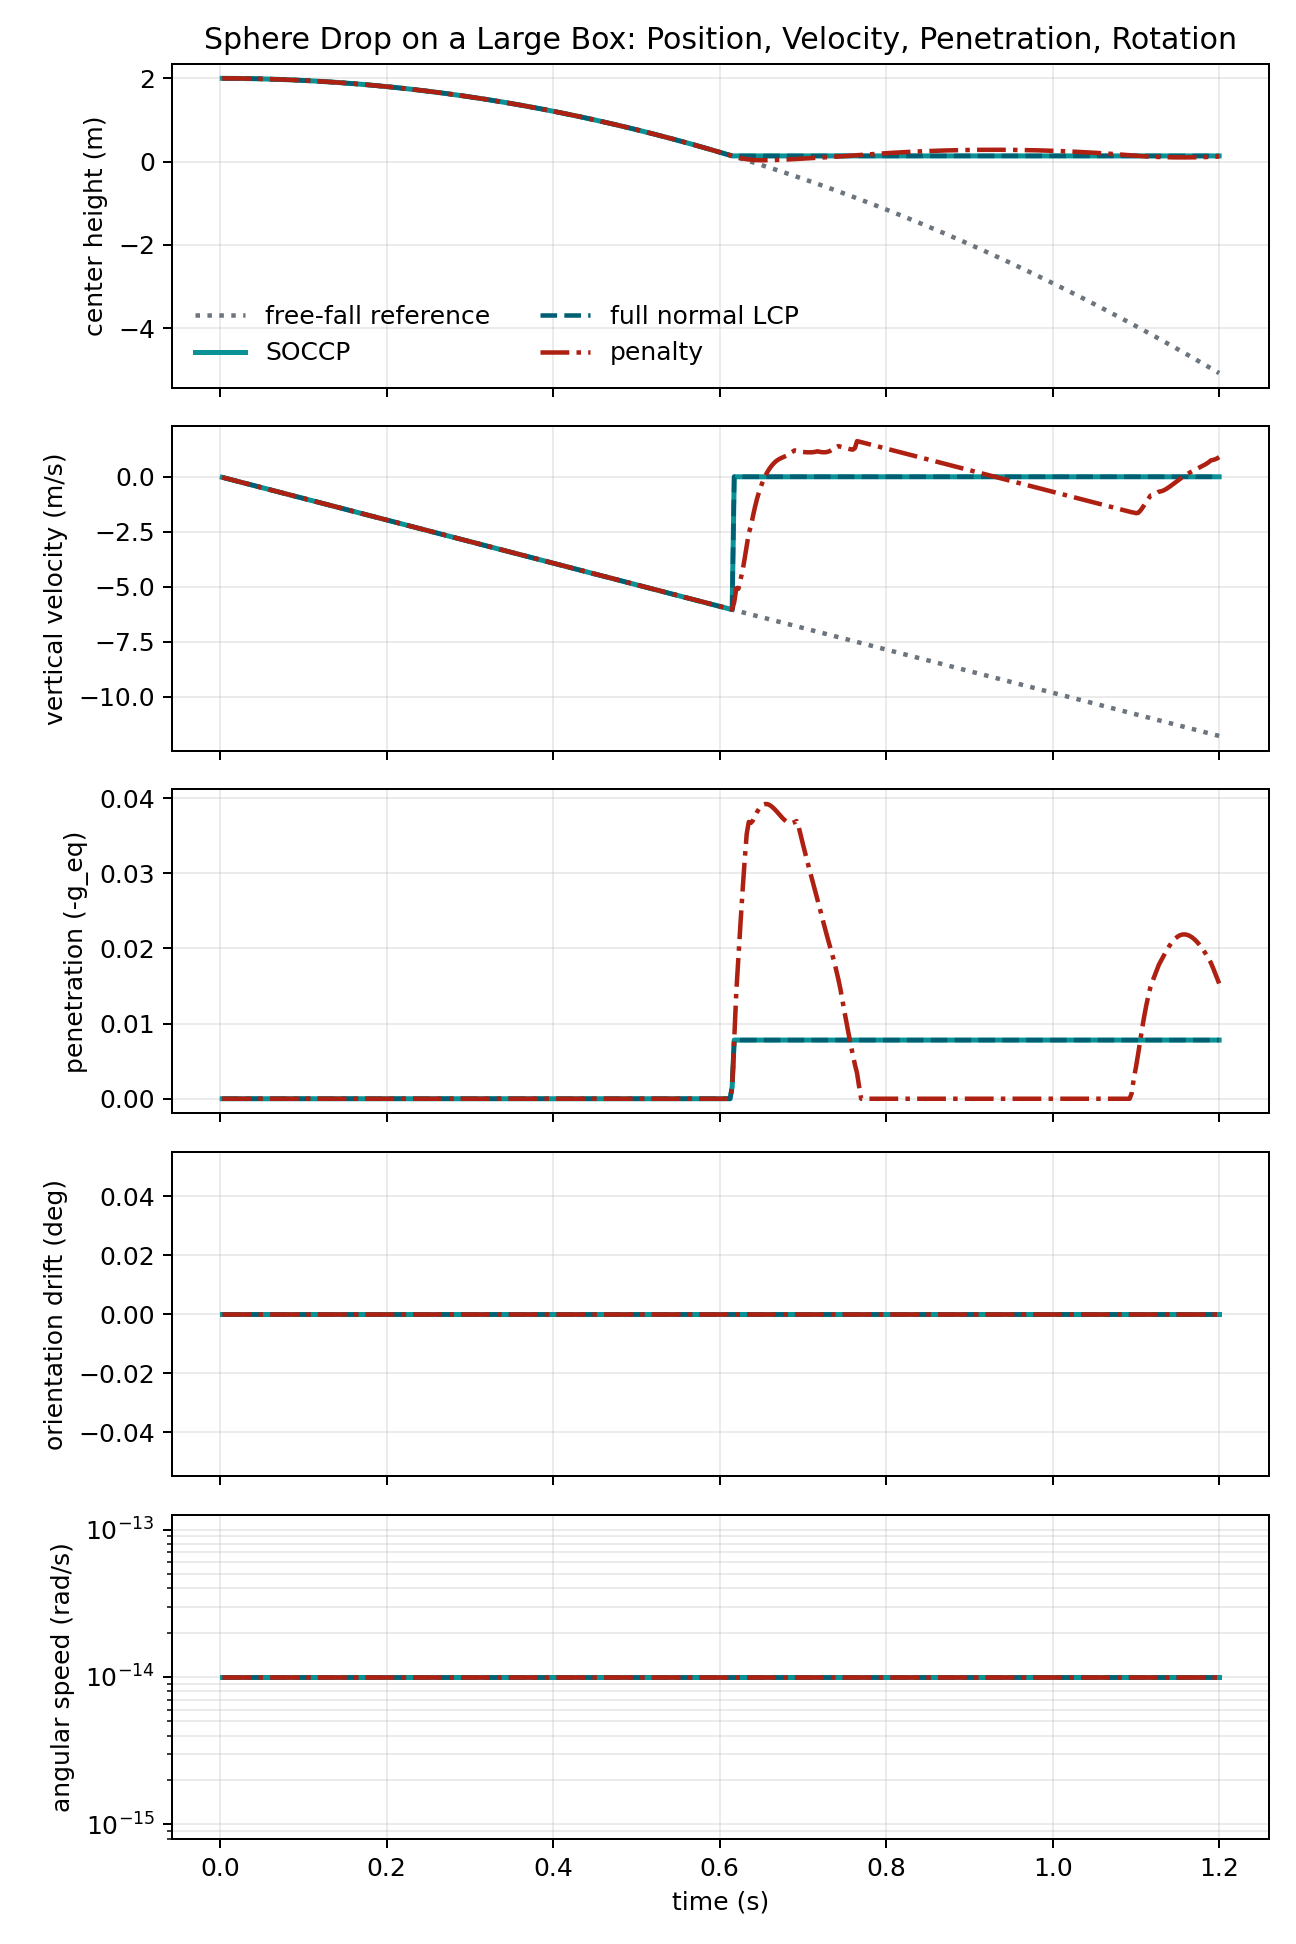
\includegraphics[width=0.80\linewidth]{../../results/benchmark_sphere_drop_compare.png}
    \caption{单球落体 sanity-check 中，解析自由落体参照、SOCCP、full normal LCP与罚函数三条分支的质心高度、竖直速度、等效穿透量、姿态漂移和角速度对比。}
    \label{fig:sphere_drop_compare}
\end{figure}

\subsection{补充 sanity-check：平动主导滑移摩擦与解析库仑参照}
\textbf{设置：} 为补足``摩擦型主链是否正确''这一最容易被质疑的环节，本文再构造一个比 oblique-box 场景更干净的补充 benchmark：只保留一个持续接触的平面约束与两个切向平动自由度，显式关闭转动与扭转载荷，并将该问题分别交给去掉扭转项后的三维SOCCP分支、一个独立实现的 friction PGS 基线，以及一个基于多面体摩擦锥近似的独立 polyhedral friction 外部基线。由于该场景退化为标准的解析库仑滑移问题，其参考解满足$v_x(t)=\max(v_0-\mu g t,0)$，位移满足$x(t)=v_0t-\tfrac12\mu g t^2$直到停止。图\ref{fig:scene_sanity_sliding_friction}给出了该 sanity-check 的模型示意：一个平动主导的小块在平面上沿$x$方向滑移，用于比较解析库仑参照、SOCCP 3D 分支、friction PGS 与 polyhedral friction 外部基线。

\begin{figure}[htbp]
    \centering
    \includegraphics[width=0.66\linewidth]{./figures/scene_sanity_sliding_friction.png}
    \caption{平动主导滑移摩擦 sanity-check 的模型示意：单个小块在平面上沿切向滑移，显式关闭转动与扭转载荷，用于比较解析库仑滑移参照、SOCCP三维摩擦分支、friction PGS 与 polyhedral friction 外部基线。}
    \label{fig:scene_sanity_sliding_friction}
\end{figure}

\textbf{结果：} 解析参考的停止时间为$0.25484$s，而SOCCP三维分支、friction PGS 与 polyhedral friction 外部基线都在$0.250$s将速度降到$0.02$m/s以下；解析停止距离为$0.12742$m，而三条数值路径都得到$0.12692$m，最大位置误差均为$4.997\times10^{-4}$m。速度曲线方面，三条数值路径对解析库仑参照的最大误差都在当前输出精度下为零；同时，三条路径在整个时程中的峰值残差都为零。法向冲量恒为$19.62$N$\cdot$s/m，对应$mg$；切向冲量恒为$-7.848$N$\cdot$s/m，对应$-\mu mg$。这说明：在显式关闭扭转载荷后，本文的三维摩擦主链不仅与独立 friction PGS 基线共同复现了标准解析库仑滑移规律，而且也与独立 polyhedral-cone 外部基线保持一致。因此，后文的 oblique-box 图不再承担``证明三维摩擦正确''的责任，而只承担``展示四维扭转载荷会改变更复杂三维动力学''的责任。

\begin{figure}[htbp]
    \centering
    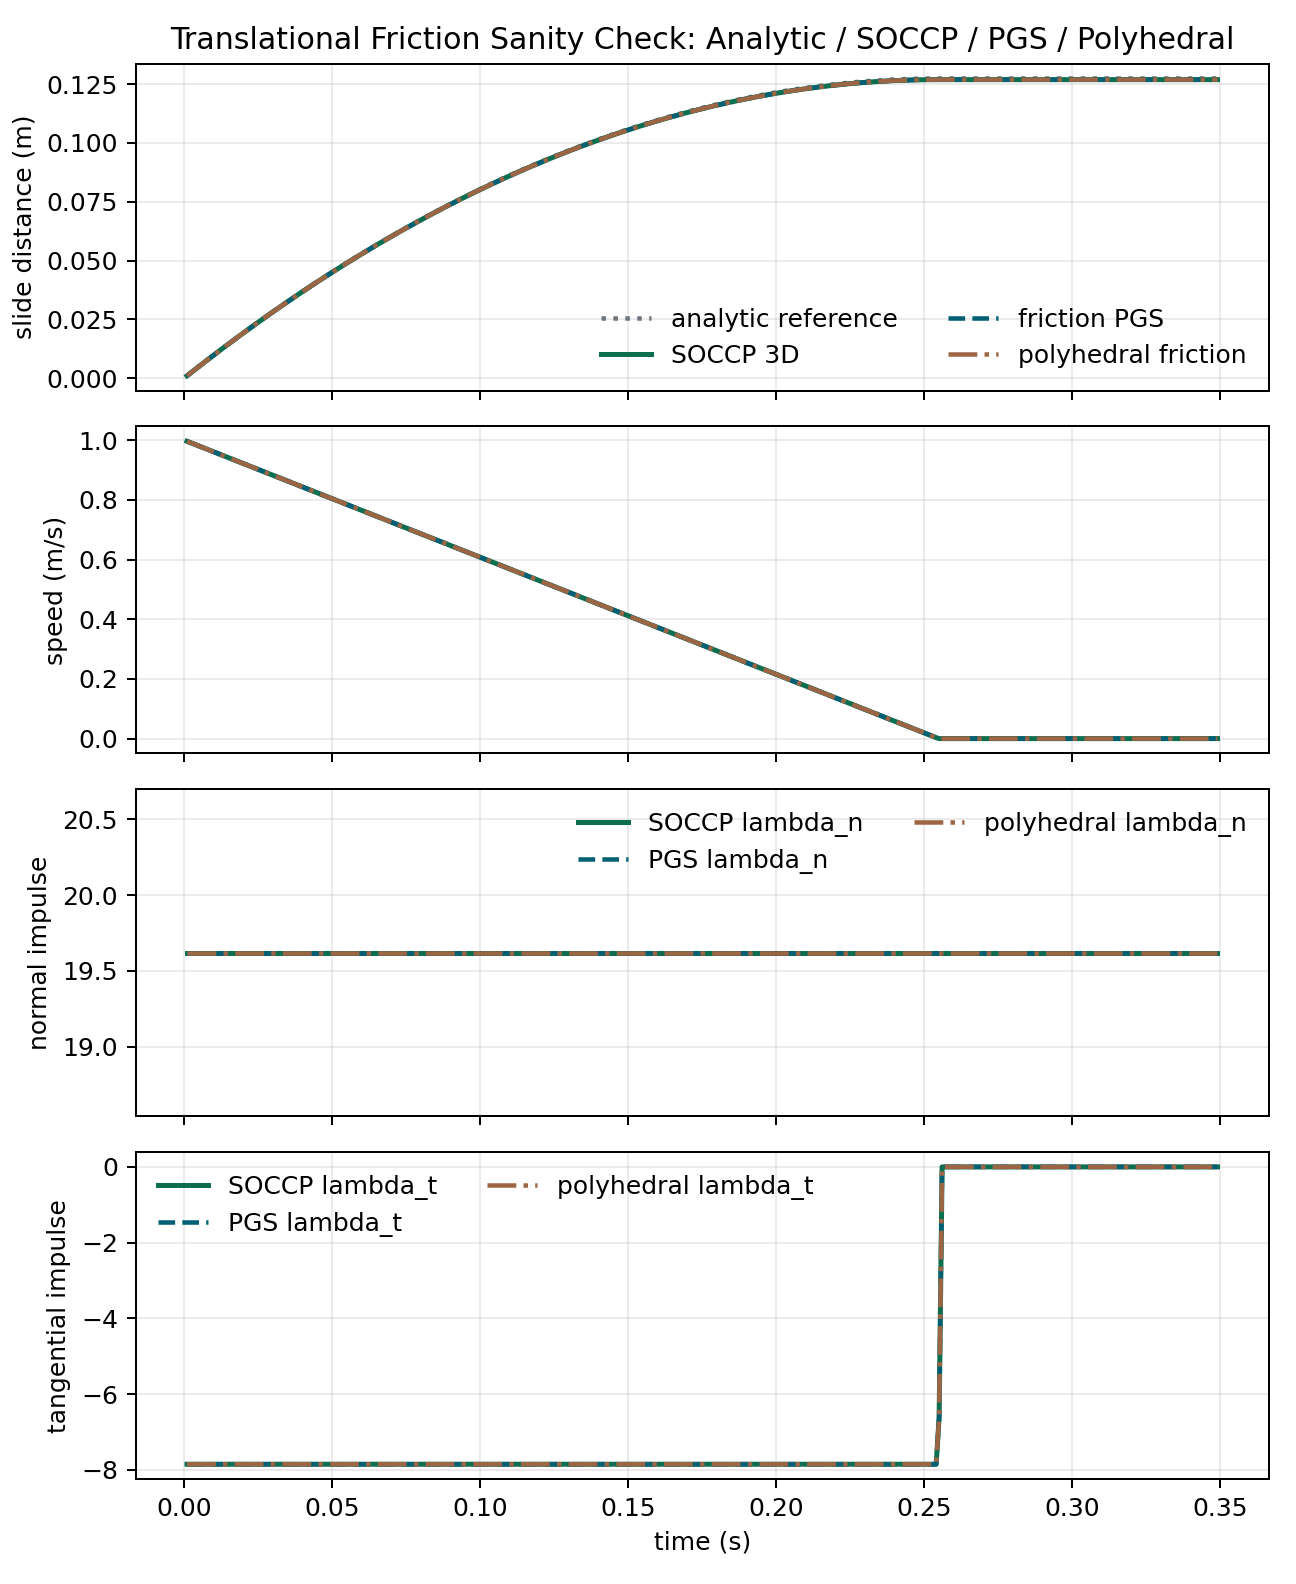
\includegraphics[width=0.80\linewidth]{../../results/benchmark_engine_sliding_friction_reference.png}
    \caption{平动主导滑移摩擦 sanity-check 中，解析库仑滑移参照、SOCCP三维摩擦分支、friction PGS 与 polyhedral friction 外部基线在位移、速度、法向冲量与切向冲量上的对比。}
    \label{fig:sliding_friction_reference}
\end{figure}

\subsection{算例一：旋转圆柱的扭转半径校准}
\textbf{设置：} 取半径$R=0.45$、高度$H=0.24$、质量$m=3.0$的圆柱体，其底面与刚性平面形成有限接触斑。由当前代码计算得到等效扭转半径$r_{\tau}$，再代入降阶扭转摩擦律
\begin{equation}
    M_{\tau}^{model} = \mu m g r_{\tau},
\end{equation}
并与经典均匀面压理论中的
\begin{equation}
    M_{\tau}^{theory} = \frac{2}{3}\mu m g R
\end{equation}
进行比较。同时引入一个点接触基线：若不使用有限接触斑诱导的$r_{\tau}$，而仍采用传统点接触近似，则在同样的降阶模型中不存在由接触斑尺度给出的扭转载荷力臂，因而该基线不产生自旋衰减。
图\ref{fig:scene_case1_cylinder_calibration}给出了该算例的模型场景：一个绕接触法线自旋的圆柱与刚性平面形成有限接触斑。

\begin{figure}[htbp]
    \centering
    \includegraphics[width=0.64\linewidth]{./figures/scene_case1_cylinder_calibration.png}
    \caption{算例一的模型场景：圆柱底面与刚性平面形成有限接触斑，并绕接触法线自旋。}
    \label{fig:scene_case1_cylinder_calibration}
\end{figure}

\textbf{结果：} 当前实现给出的等效扭转半径为$r_{\tau}=0.3120$，而经典有效力臂为$\frac{2R}{3}=0.3000$，相对误差为$4.00\%$。据此得到的停止时间分别为$t_{stop}^{model}=0.9451$s 与 $t_{stop}^{theory}=0.9830$s，相对误差为$3.85\%$。图\ref{fig:cylinder_spin}中同时给出了点接触基线，其角速度在整个过程中保持初值不变。这说明：若不把有限接触斑压缩为一个有效扭转尺度，经典点接触近似无法在同一降阶模型中恢复阻转效应；而本文几何压缩映射则能以较小误差恢复经典圆盘阻转时间尺度。

\begin{figure}[htbp]
    \centering
    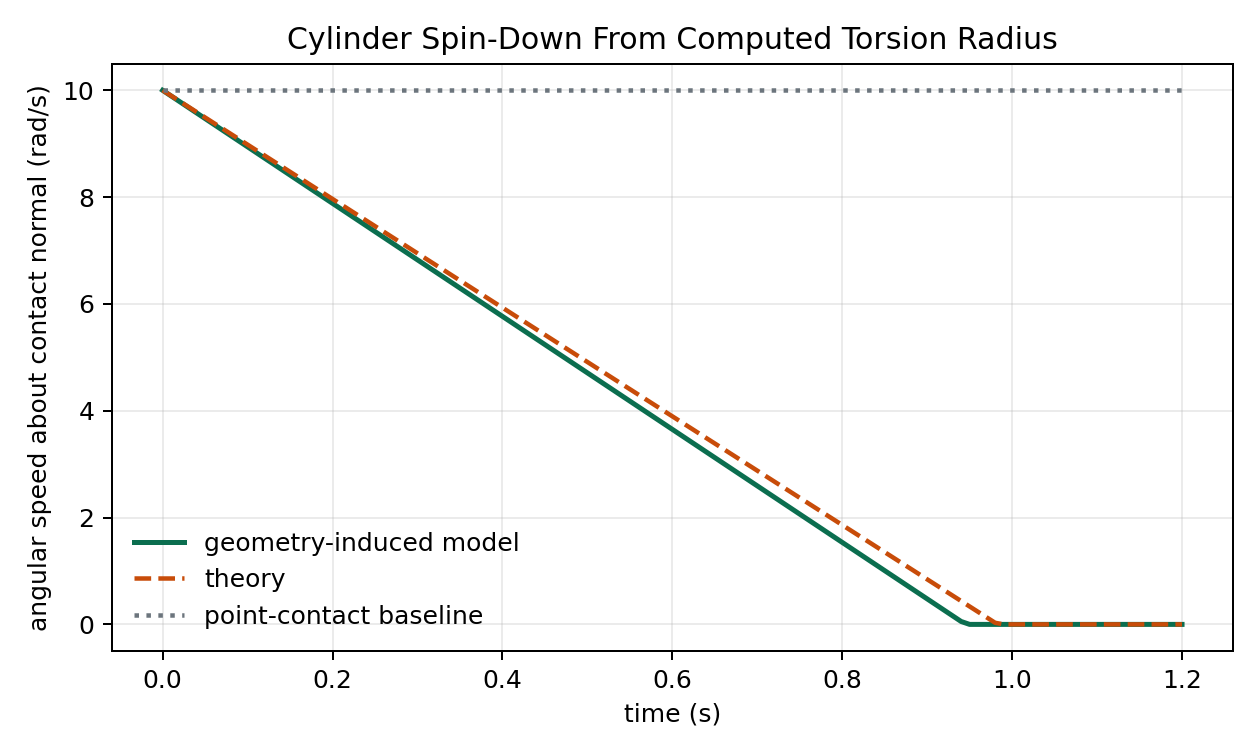
\includegraphics[width=0.78\linewidth]{../../results/benchmark_cylinder_spin.png}
    \caption{由代码计算的等效扭转半径诱导的圆柱自旋衰减曲线。图中同时给出经典理论线性衰减结果以及不含接触斑扭转尺度的点接触基线。}
    \label{fig:cylinder_spin}
\end{figure}

\subsection{补充 sanity-check：受控扭转载荷与解析参考}
\textbf{设置：} 上一小节回答的是``几何压缩得到的扭转尺度是否合理''，但它仍然属于几何量标定。为把四维摩擦主链从``会产生动力学差异''推进到``可与解析参考闭环''，本文额外构造一个更干净的受控 benchmark：保持固定接触几何、只保留一个法向约束和一个绕接触法线的自旋自由度，并取扭转半径$\hat r_{\tau}=0.30$，从而得到解析参考
\begin{equation}
    \omega(t)=\max\left(\omega_0-\frac{\mu m g \hat r_{\tau}}{I_y}t,0\right).
\end{equation}
在同一离散步长下，对比三条路径：解析参考、启用扭转载荷的SOCCP四维分支，以及强制$\lambda_{\tau}=0$的三维基线。该算例不再依赖全引擎几何演化，而是专门隔离``4D锥+半光滑牛顿''本身是否给出正确的阻转力学。图\ref{fig:scene_sanity_torsion_reference}给出了该受控扭转载荷 sanity-check 的模型示意。

\begin{figure}[htbp]
    \centering
    \includegraphics[width=0.66\linewidth]{./figures/scene_sanity_torsion_reference.png}
    \caption{受控扭转载荷 sanity-check 的模型示意：固定接触几何下的圆柱自旋问题，用于比较解析扭转阻尼参考、SOCCP四维分支与去扭转三维基线。}
    \label{fig:scene_sanity_torsion_reference}
\end{figure}

\textbf{结果：} 解析参考给出的停止时间为$0.9830$s，SOCCP四维分支的停止时间为$0.9400$s，相对误差为$4.37\%$；而去掉扭转载荷后的三维基线在整个$1.2$s窗口内都未停止。更关键的是，SOCCP四维分支在整个激活阶段对解析角速度曲线的最大误差小于$10^{-13}$，法向载荷误差小于$10^{-12}$，扭转载荷误差也小于$10^{-12}$；累计自旋角误差仅为$4.99\times10^{-2}$rad。这说明：在把接触几何冻结为受控参考后，本文的四维摩擦锥与SOCCP/半光滑牛顿主链能够精确复现解析扭转阻尼规律。因此，后文的全引擎圆柱与oblique-box算例应被解释为``四维扭转载荷会改变完整动力学''的证据，而不再承担``独立证明4D分支正确''的责任。

\begin{figure}[htbp]
    \centering
    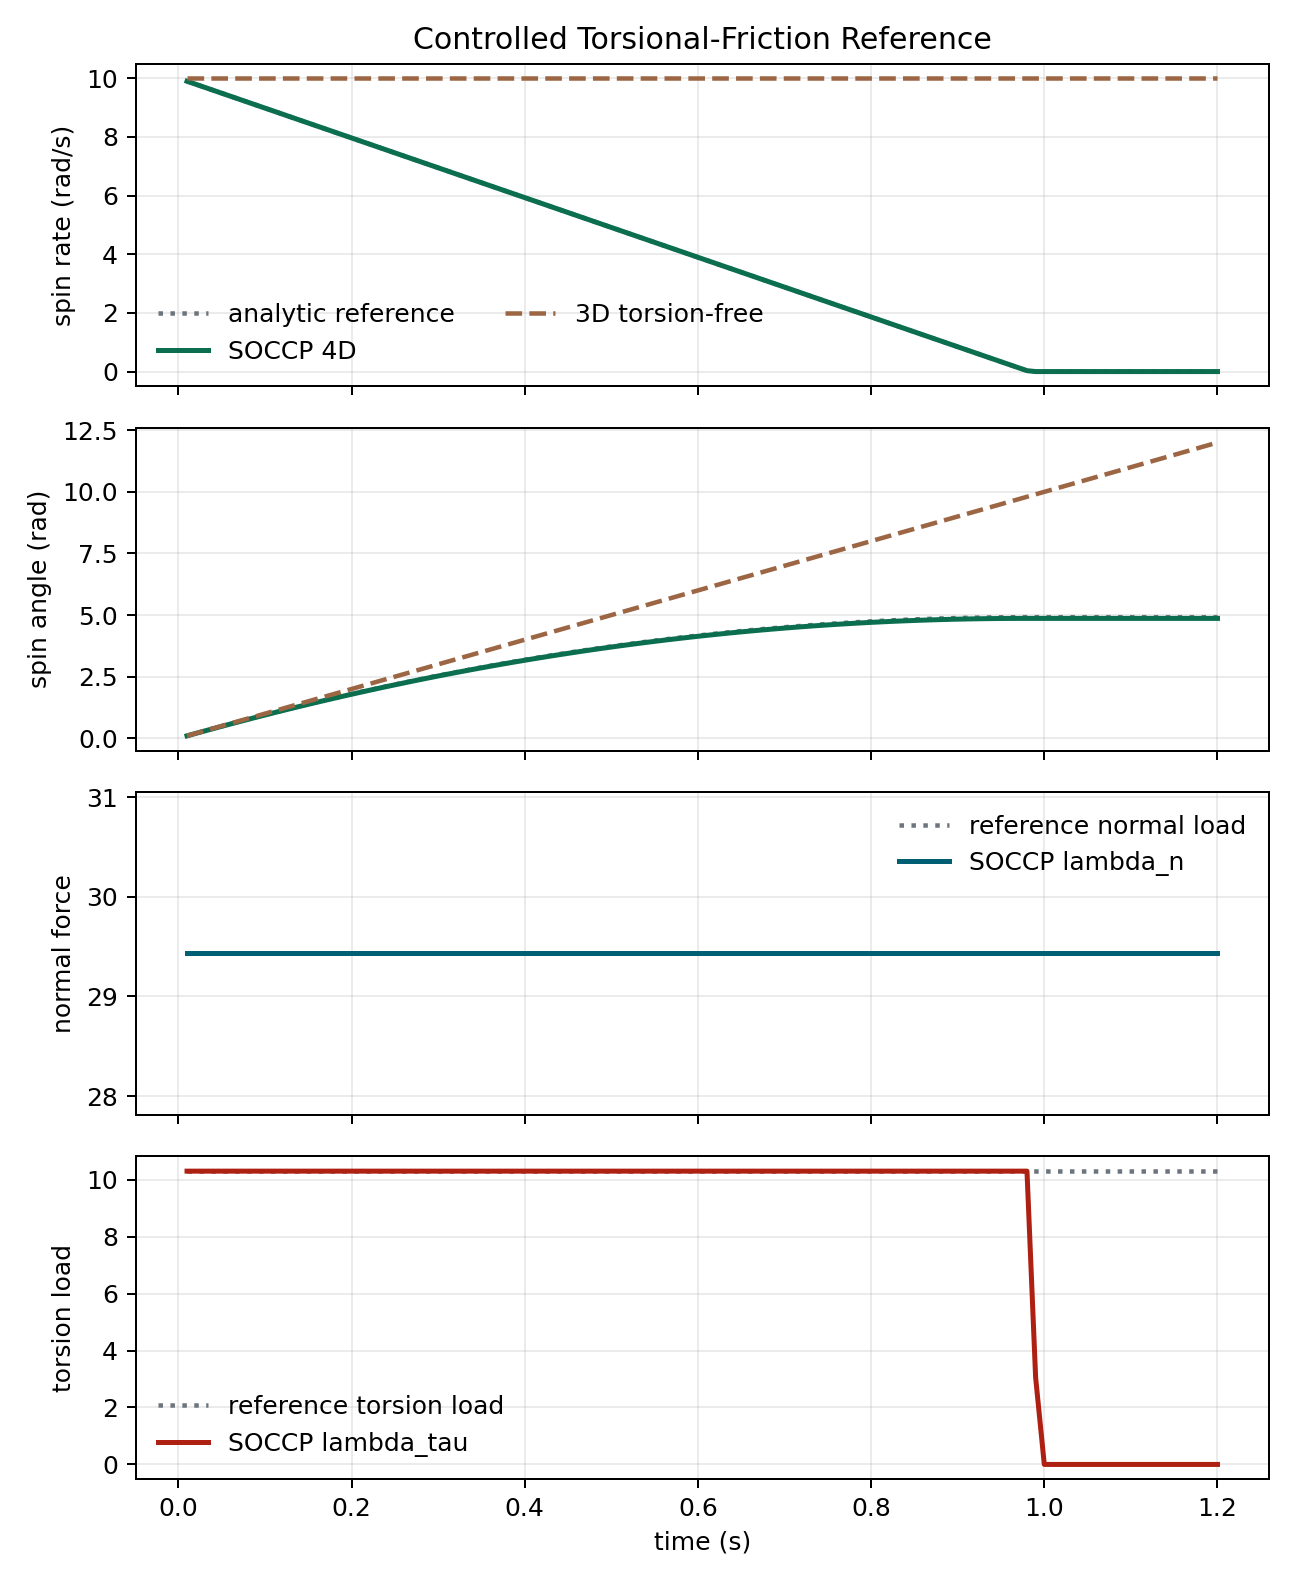
\includegraphics[width=0.80\linewidth]{../../results/benchmark_torsion_friction_reference.png}
    \caption{受控扭转载荷 sanity-check 中，解析参考、SOCCP四维分支与去扭转三维基线在角速度、自旋角、法向载荷与扭转载荷上的对比。}
    \label{fig:torsion_friction_reference}
\end{figure}

\subsection{补充 solver cross-check：耦合平动-扭转状态下的SOCCP 4D与独立4D PGS对照}
\textbf{设置：} 受控扭转载荷算例已经说明``4D锥+SOCCP''能够精确复现解析阻转规律，但它仍只激活了法向约束与一个扭转自由度。为进一步回应``当切向平动、yaw与扭转载荷同时激活时，4D响应是否仍然可信''这一质疑，本文再构造一个固定接触几何的耦合参考：保持单一有限接触斑不变，让刚体同时具有$v_x$、$v_z$和$\omega_y$三个自由度，并在完全相同的质量矩阵、摩擦系数、切向-扭转雅可比与时间步下，分别交给SOCCP四维分支和一个独立实现的4D projected Gauss--Seidel（4D PGS）求解。该算例不再依赖全引擎几何演化，因此其定位不是取代后续的全引擎圆柱/oblique-box场景，而是在``受控扭转解析参考''与``全引擎行为差异图''之间插入一层\textbf{独立求解器交叉验证}。图\ref{fig:scene_sanity_4d_coupled_reference}给出了该固定接触斑下的耦合平动-扭转参考场景。

\begin{figure}[htbp]
    \centering
    \includegraphics[width=0.68\linewidth]{./figures/scene_sanity_4d_coupled_reference.png}
    \caption{耦合平动-扭转4D参考场景：固定接触斑下同时激活$v_x$、$v_z$与$\omega_y$，用于比较SOCCP四维分支与独立4D PGS。}
    \label{fig:scene_sanity_4d_coupled_reference}
\end{figure}

\textbf{结果：} 在这一固定接触斑 benchmark 中，SOCCP与独立4D PGS得到完全一致的法向载荷，末态自旋都衰减到零；两条路径的scaled residual与锥互补违约在整个时程内都降到机器精度量级。更重要的是，在所有三个摩擦自由度同时激活的情况下，两者给出的时域响应仍保持一致趋势：最大$ v_x / v_z / \omega_y $差分别为$3.39\times10^{-2}$、$1.83\times10^{-2}$和$4.02\times10^{-2}$，累计滑移差为$1.57\times10^{-2}$m，yaw角差为$1.68\times10^{-2}$rad。与此同时，最大切向-扭转载荷差为$1.214$，说明这两条独立4D求解路径并未达到 machine-precision 轨迹重合；但它们已经足以共同表明：\textbf{当切向平动、yaw与扭转载荷同时存在时，当前4D主链给出的动力学趋势并非某一SOCCP实现的数值产物，而能被另一条独立4D projected solver重复得到。} 这条证据因此补上了``受控扭转参考很强，但仍然太单自由度''的缺口。

\begin{figure}[htbp]
    \centering
    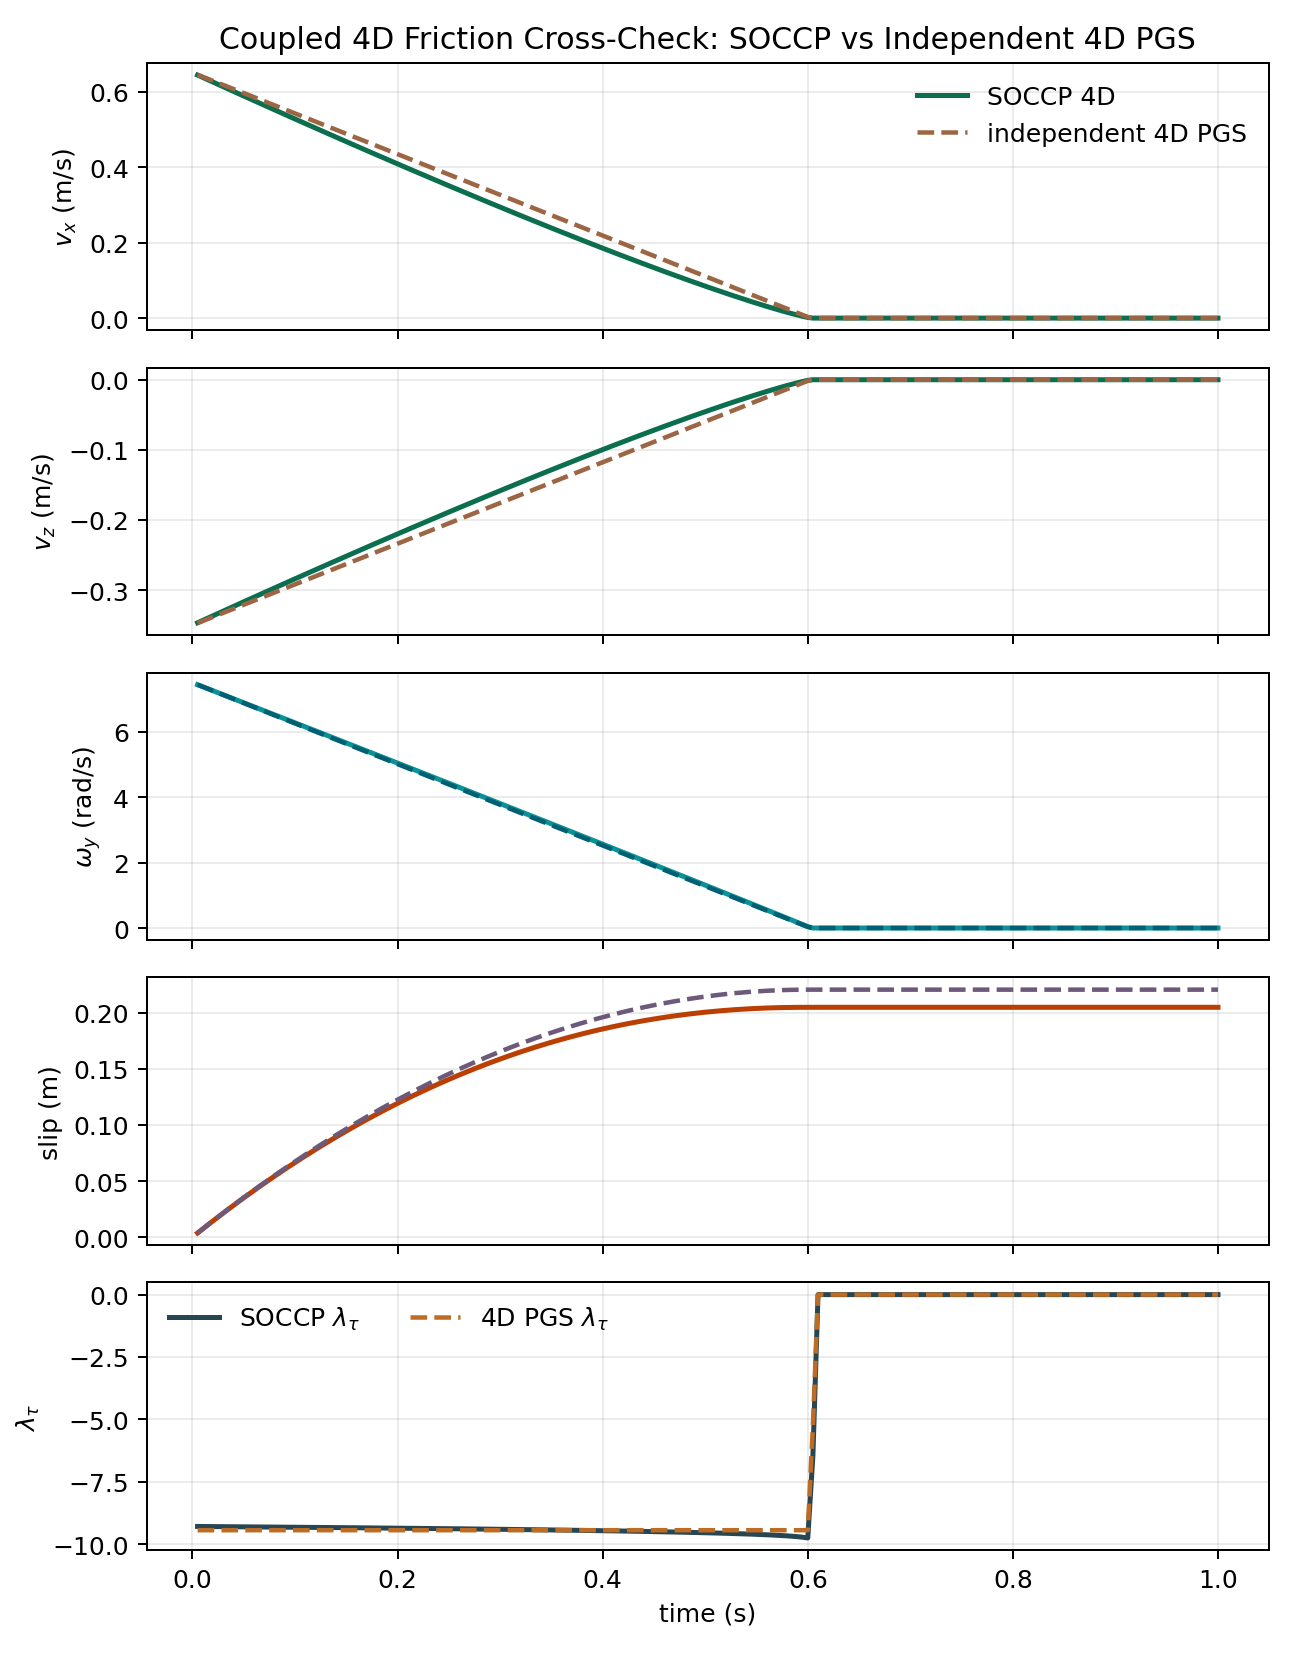
\includegraphics[width=0.80\linewidth]{../../results/benchmark_4d_coupled_friction_reference.png}
    \caption{耦合平动-扭转4D solver cross-check 中，SOCCP四维分支与独立4D PGS在$v_x$、$v_z$、$\omega_y$、累计滑移和$\lambda_{\tau}$上的对比。该图不以解析解为参照，而以独立4D projected solver作为交叉验证。}
    \label{fig:coupled_4d_reference}
\end{figure}

\subsection{算例二：全引擎4D friction与3D基线的自旋衰减对比}
\textbf{设置：} 前面几小节已经分别给出了几何扭转尺度的校准证据、固定接触几何下的4D正确性证据以及独立4D solver cross-check，但它们仍不足以回答``四维摩擦锥在完整时域主链里是否真的起作用''。为此，本文进一步构造一个全引擎 benchmark：保持同一圆柱--平面SDF几何、同一SOCCP主链、同一摩擦系数与时间积分参数，仅改变摩擦律维数。其一，采用本文的四维摩擦锥，使切向两自由度与扭转载荷在同一锥内联合演化；其二，构造一个去掉扭转分量的三维基线，即保留相同法向与二维切向库仑摩擦，但强制$\lambda_\tau=0$。
图\ref{fig:scene_case2_torsion_compare}给出了该对比算例的模型场景。两条路径使用完全相同的圆柱--平面几何与时间积分设置，只在扭转载荷自由度上存在差别。

\begin{figure}[htbp]
    \centering
    \includegraphics[width=0.88\linewidth]{./figures/scene_case2_torsion_compare.png}
    \caption{算例二的模型场景：同一圆柱--平面全引擎自旋问题，左侧为启用扭转载荷的四维摩擦模型，右侧为强制$\lambda_\tau=0$的三维基线。}
    \label{fig:scene_case2_torsion_compare}
\end{figure}

\textbf{结果：} 在相同初始自旋条件下，四维摩擦模型在$t=0.31$s时已将圆柱自旋衰减至$0.5$rad/s以下，并在$1.2$s时将角速度降至$1.58\times 10^{-5}$rad/s；相比之下，去掉扭转载荷后的三维基线在$1.2$s时仍保留$2.19$rad/s的角速度。换言之，在该全引擎算例中，四维摩擦锥相对于三维基线额外消除了$99.999\%$的残余自旋。结合上一小节的受控解析参考，这一结果更准确地应被理解为：四维摩擦主链不仅在固定接触几何下可对照解析阻转规律，而且在完整SOCCP时域链中也会转化为可观测的动力学差异。

\begin{figure}[htbp]
    \centering
    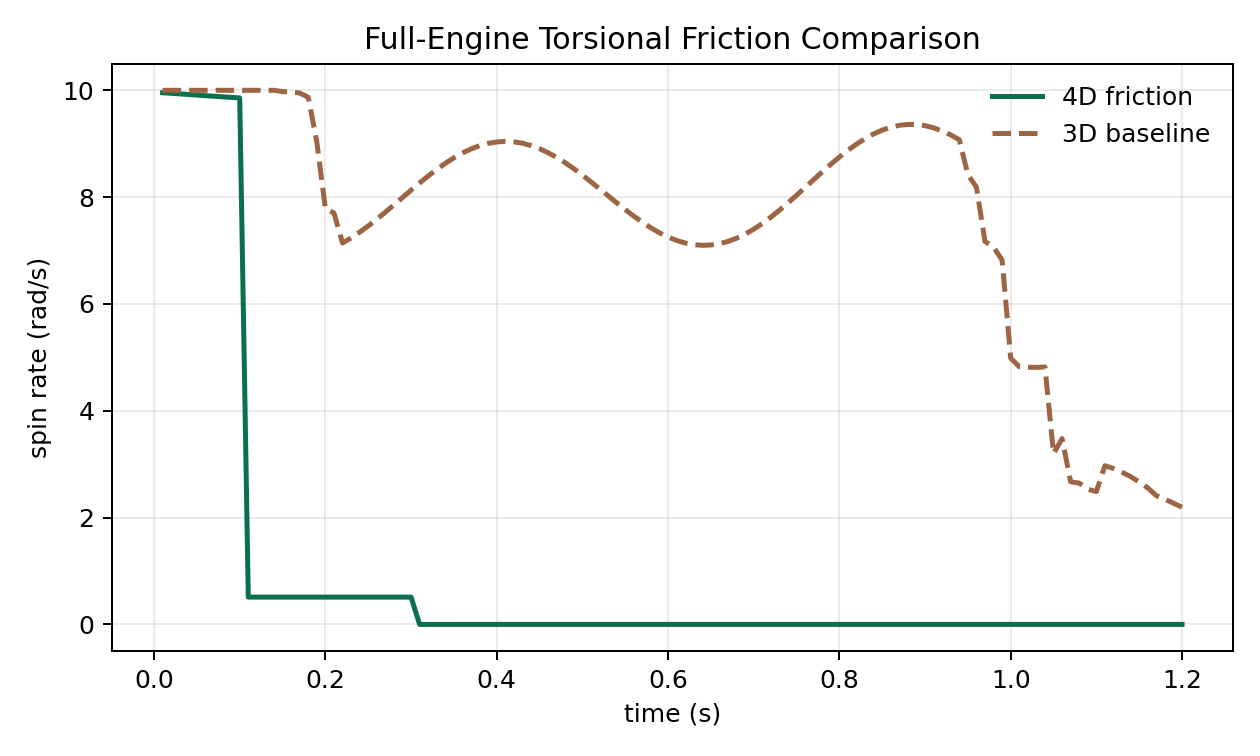
\includegraphics[width=0.78\linewidth]{../../results/benchmark_engine_torsion_compare.png}
    \caption{全引擎圆柱自旋算例中，四维摩擦锥与去掉扭转项的三维基线对比。四维模型快速耗散绕接触法线的自旋，而三维基线保留了显著残余角速度。}
    \label{fig:torsion_compare}
\end{figure}

\subsection{算例三：尖锐角特征的受控下压与分辨率收敛}
\textbf{设置：} 为避免接触动力学瞬态对几何结论的掩盖，本文采用一枚绕$x$轴与$z$轴各旋转$45^\circ$后的立方体尖角作为``尖锐物''，沿法向以受控路径压向刚性平面。对固定路径分别取$p=2,4,6$，直接计算$g_{eq}^{(p)}$随下压过程的变化。
图\ref{fig:scene_case3_sharp_corner}给出了该算例的模型场景：旋转后的立方体尖角沿法向受控压向刚性平面。

\begin{figure}[htbp]
    \centering
    \includegraphics[width=0.64\linewidth]{./figures/scene_case3_sharp_corner.png}
    \caption{算例三的模型场景：绕$x$轴和$z$轴各旋转$45^\circ$后的立方体尖角，沿法向以受控路径压向刚性平面。}
    \label{fig:scene_case3_sharp_corner}
\end{figure}

\textbf{结果：} 在相同的终端尖角压入量下，等效穿透量$-g_{eq}^{(p)}$随$p$单调增大：当$p=2,4,6$时，其终值分别为$1.072\times 10^{-2}$、$1.230\times 10^{-2}$和$1.319\times 10^{-2}$。相较于$p=2$，$p=4$与$p=6$对应的终端等效穿透量分别提高了$14.8\%$和$23.0\%$。这与第2节和第4节关于``高阶矩比对局部深穿透区域具有更强聚焦能力''的理论结论一致。

与此同时，本文增加了一个针对同一尖角场景的分辨率收敛对比。以$128^3$均匀体素结果作为参考解，考察$p=2$与$p=6$在不同网格下的$g_{eq}$相对误差。结果表明：$16^3$网格会直接漏检该尖角接触；当分辨率提高到$64^3$时，$p=2$对应的相对间隙误差约为$8.15\%$，而$p=6$仍约为$29.7\%$。因此，本工作关于$p$的聚焦结论是成立的，但高阶$p$确实更依赖细网格或自适应积分。基于这一结果，本文在当前投稿中明确收窄数值主张：对于均匀体素原型，仅将$p=2$作为默认稳健参数、将$p=4$作为较细网格下的可选增强，而将$p=6$仅保留为展示理论趋势的高阶示例，不声称其已成为当前实现中的工程默认配置。这也解释了为何本文将均匀体素实现视为原型基线，而把八叉树细化保留为后续工作。

\begin{figure}[htbp]
    \centering
    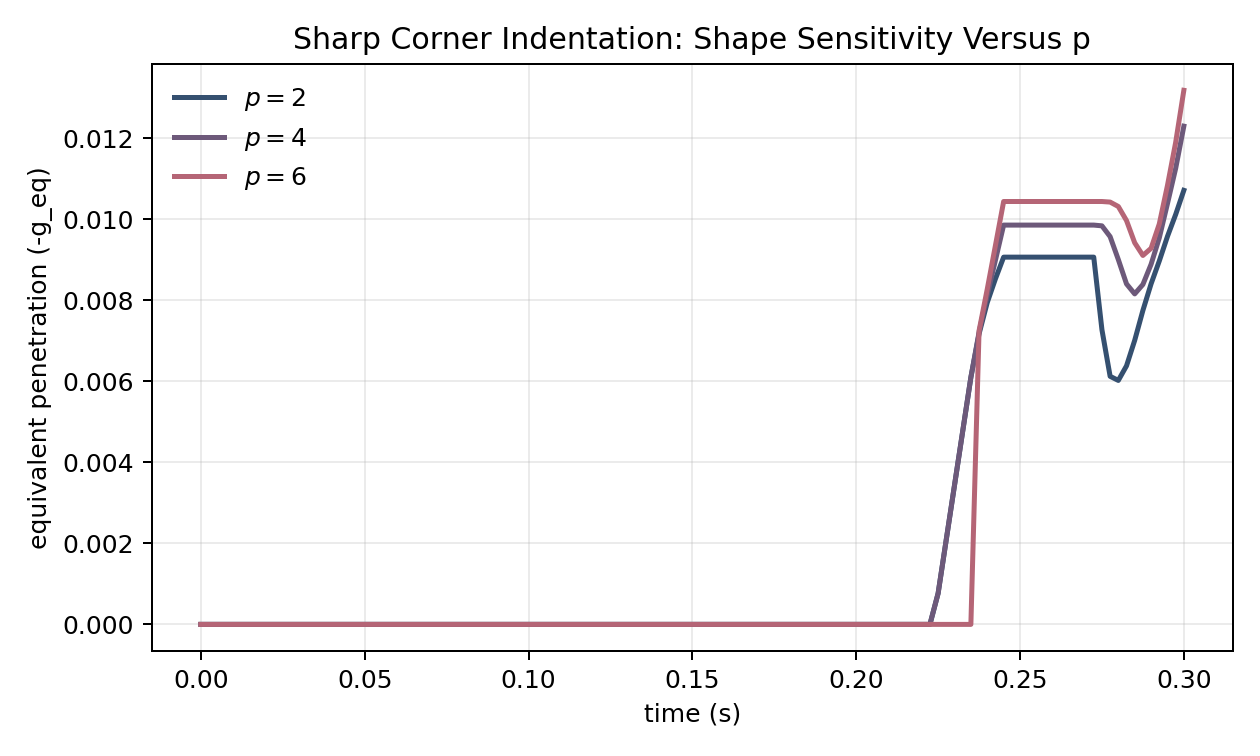
\includegraphics[width=0.78\linewidth]{../../results/benchmark_sharp_drop.png}
    \caption{受控尖角下压过程中，不同$p$值对应的等效穿透量时程。随着$p$增大，曲线终值单调提高，显示出更强的尖锐特征聚焦。}
    \label{fig:sharp_drop}
\end{figure}

\begin{figure}[htbp]
    \centering
    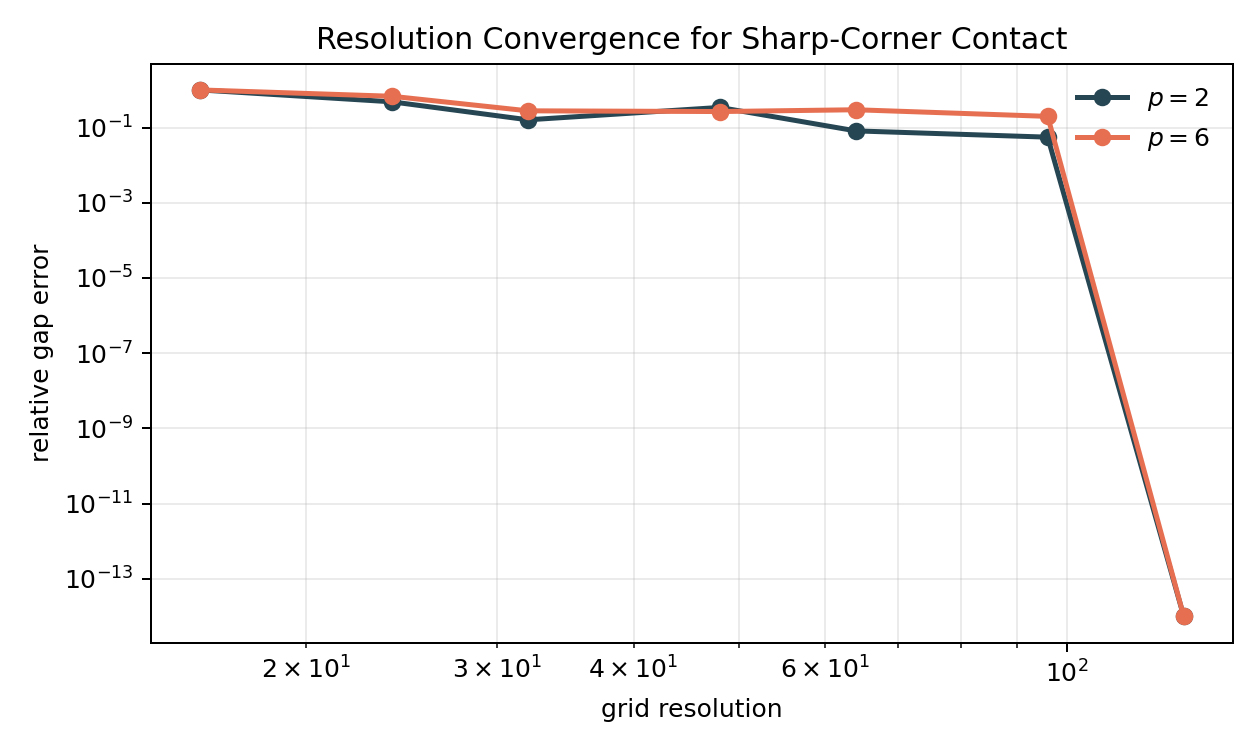
\includegraphics[width=0.78\linewidth]{../../results/benchmark_resolution_convergence.png}
    \caption{尖角接触场景下，均匀体素积分对$g_{eq}$的分辨率收敛行为。高阶$p$对局部峰值更敏感，但也更依赖细网格分辨率。}
    \label{fig:resolution_convergence}
\end{figure}

\subsection{算例四：对称两接触normal-only场景中的三路一致性检查}
\textbf{设置：} 取``上箱体--下箱体--地面''构成的两接触堆叠系统，分别采用本文的SDF体积接触$+$全局SOCCP主链、一个完整引擎级的全局法向LCP分支（full normal LCP），以及一个基于相同SDF接触几何但使用罚函数求解的基线模型进行时域积分。该场景关闭摩擦与扭转载荷，且几何与初始条件保持轴对称，因此它更适合作为``SOCCP在normal-only极限下是否正确退化为法向LCP''的一致性检查，而不是一个刻意放大方法差异的压力测试。比较指标为整个过程中的最大等效穿透量与接触阶段的求解残差。
图\ref{fig:scene_case4_multicontact_stack}给出了该两接触堆叠算例的模型场景：上箱体与下箱体形成第一处接触，下箱体与地面形成第二处接触。

\begin{figure}[htbp]
    \centering
    \includegraphics[width=0.68\linewidth]{./figures/scene_case4_multicontact_stack.png}
    \caption{算例四的模型场景：上箱体--下箱体--地面构成的两接触堆叠系统，用于比较SOCCP、full normal LCP与罚函数三条分支在对称normal-only极限下的一致性。}
    \label{fig:scene_case4_multicontact_stack}
\end{figure}

\textbf{结果：} 在当前参数下，SOCCP、full normal LCP与罚函数三条分支的峰值等效穿透量都为$2.963\times 10^{-2}$；其中SOCCP与full normal LCP之间的峰值差在当前输出精度下为零。图\ref{fig:engine_multicontact}显示，三条穿透曲线在该对称normal-only场景中基本重合，这正是理论上应当出现的退化结果：当摩擦与扭转载荷关闭、接触又保持法向对称时，SOCCP主链应退化为纯法向全局LCP，而当前代码确已复现这一极限。求解器统计方面，SOCCP分支的峰值残差为$2.89\times 10^{-1}$、单步最多$17$次牛顿迭代；full normal LCP分支的峰值残差为$2.89\times 10^{-1}$，单步最多使用$160$次投影Gauss--Seidel迭代。因而，这一算例在本文中的定位不再是``SOCCP优于罚函数''，而是``SOCCP、引擎级法向LCP与罚函数在对称normal-only极限下给出一致宏观响应''，从而为后续更强三维场景中的差异化结果提供一个干净的基线参照。

\begin{figure}[htbp]
    \centering
    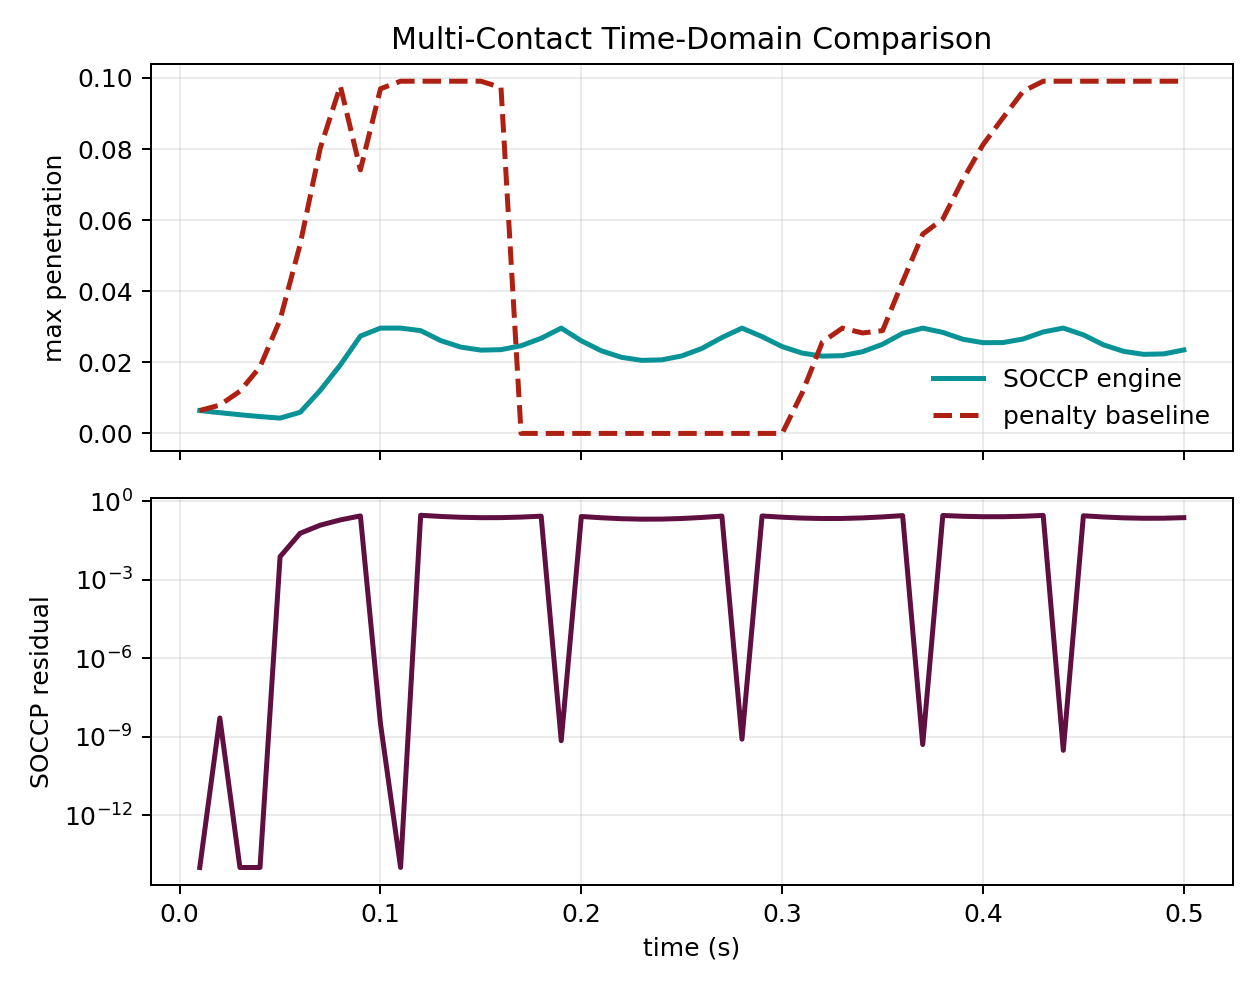
\includegraphics[width=0.78\linewidth]{../../results/benchmark_engine_multicontact.png}
    \caption{两接触堆叠时域算例中，SOCCP、full normal LCP与罚函数三条分支的最大穿透量对比，以及两条互补分支的残差与迭代时程。该图主要用作对称normal-only极限下的 solver-consistency check。}
    \label{fig:engine_multicontact}
\end{figure}

\subsection{算例五：受控二接触问题的质量比扫描}
\textbf{设置：} 考察一个由``上球--下球--地面''构成的二接触堆叠SOCCP，其中上下球质量比分别取$1:1$、$10:1$、$100:1$和$1000:1$，统一采用大时间步$h=0.05$s。该实验直接检验全局SOCCP与半光滑牛顿迭代对病态质量矩阵的敏感性。
图\ref{fig:scene_case5_mass_ratio}给出了该质量比扫描算例的模型场景：上方重球、下方轻球与地面构成两个法向接触，质量比在不同试验中变化。

\begin{figure}[htbp]
    \centering
    \includegraphics[width=0.66\linewidth]{./figures/scene_case5_mass_ratio.png}
    \caption{算例五的模型场景：上球--下球--地面构成的二接触堆叠问题，其中上下球质量比在$1$到$1000$之间变化。}
    \label{fig:scene_case5_mass_ratio}
\end{figure}

\textbf{结果：} 在所测试的四个质量比下，求解器均成功收敛，且都在$6$步牛顿迭代内达到机器精度量级的残差。也就是说，在这个受控二接触堆叠问题上，从$1$提升到$1000$的质量比并未破坏SOCCP/Fischer--Burmeister/半光滑牛顿链条的收敛性。该结果与上一小节的时域对比一起说明：当前主链在受控低维问题上具有良好局部求解鲁棒性，而在完整时域仿真中仍需要进一步改进全局化策略与接触激活阶段的数值平滑。

\begin{figure}[htbp]
    \centering
    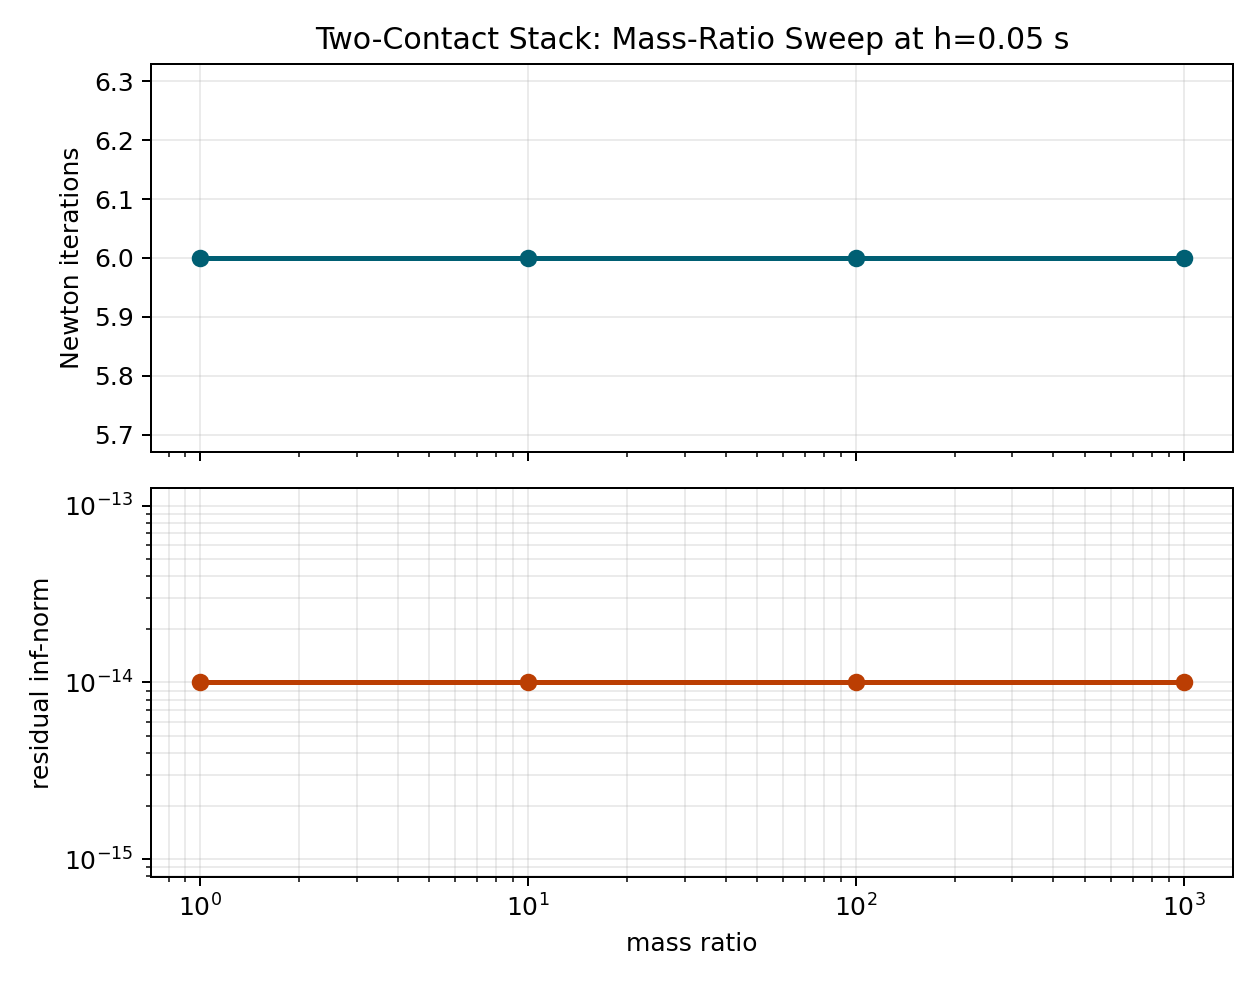
\includegraphics[width=0.78\linewidth]{../../results/benchmark_mass_ratio_stack.png}
    \caption{二接触堆叠基准中，质量比从$1$到$1000$变化时的半光滑牛顿迭代步数与残差。当前实现中四组算例均在$6$步内收敛。}
    \label{fig:mass_ratio_stack}
\end{figure}

\subsection{算例六：三支撑台上的3D tripod landing stress test}
\textbf{设置：} 为补足比``两接触堆叠''更强的三维证据，本文构造一个倾斜长方体落向三个静止支撑台的时域算例。三个支撑台在水平面内呈三角形分布，顶层长方体同时具有绕$x$轴与$z$轴的初始倾角，因此接触进入后会出现三处非共线接触、姿态耦合与接触拓扑切换。该场景当前仍关闭摩擦，因此其主要定位是 normal-only 的3D稳定性测试。相较上一版，本文在这一算例中\textbf{重新加入了full normal LCP分支}，使图\ref{fig:tripod_landing}重新回到``SOCCP / NormalLCP / tuned penalty''三路同场景对比。为回应罚函数公平性质疑，本文对罚函数路径采用\textbf{固定时间步的透明调参协议}：在相同$\Delta t=0.01$s下，对$k\in\{2\times10^4,3\times10^4,4.5\times10^4,6\times10^4,8\times10^4,10^5\}$与$c\in\{60,90,105,120,150,180\}$做扫描，并以``峰值穿透$+$姿态罚项''的固定目标函数选取最优稳定参数。最终最优参数为$k=10^5,c=150$。图\ref{fig:scene_case6_tripod}给出了该3D tripod landing stress test的模型场景：一个带初始倾角的长方体落向三个静止支撑台。

\begin{figure}[htbp]
    \centering
    \includegraphics[width=0.74\linewidth]{./figures/scene_case6_tripod.png}
    \caption{算例六的模型场景：倾斜长方体落向三个呈三角形分布的静止支撑台，用于检验三维姿态耦合与三点同时接触下的主链稳定性。}
    \label{fig:scene_case6_tripod}
\end{figure}

\begin{figure}[htbp]
    \centering
    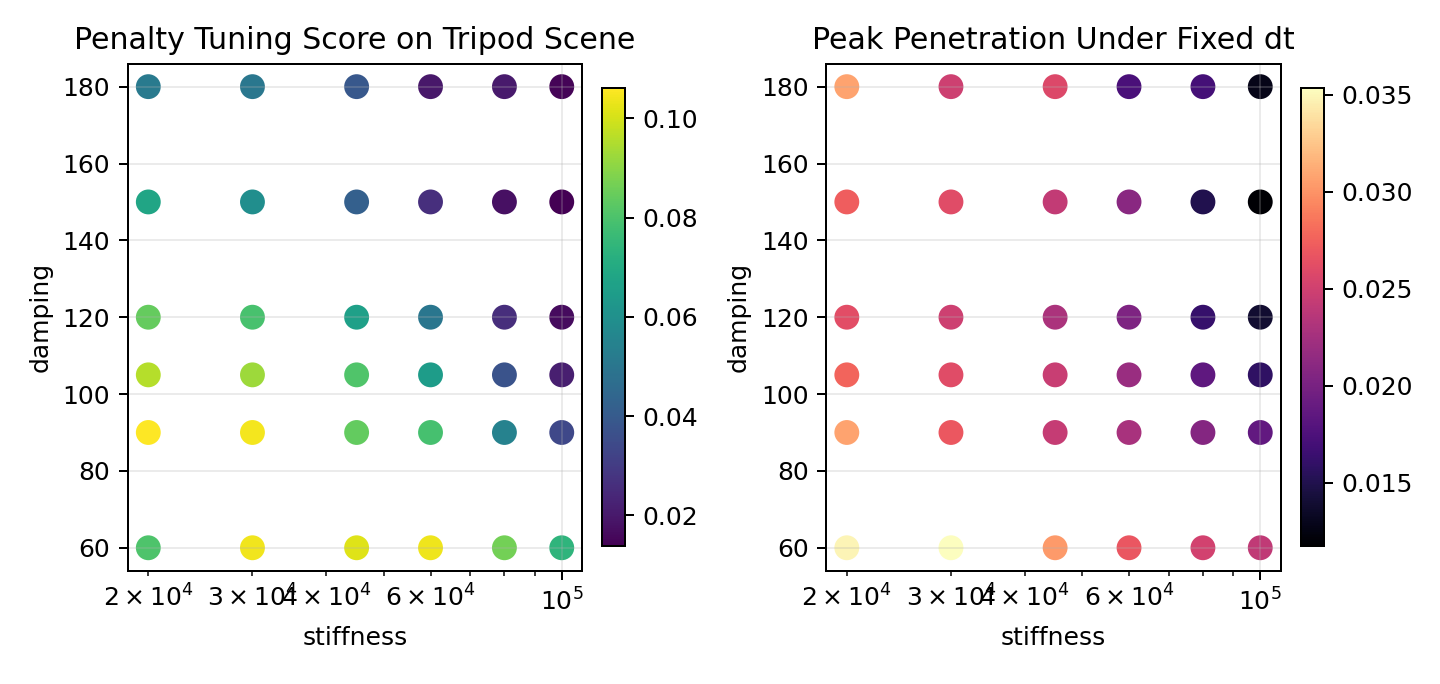
\includegraphics[width=0.78\linewidth]{../../results/benchmark_penalty_tripod_tuning.png}
    \caption{算例六中罚函数基线的透明调参结果：在固定时间步协议下扫描$k$与$c$，并以峰值穿透与姿态罚项组成的固定目标函数选取最优稳定参数。}
    \label{fig:tripod_penalty_tuning}
\end{figure}

\textbf{结果：} 在该3D tripod算例中，SOCCP与full normal LCP两条互补分支的峰值等效穿透量分别为$6.392\times10^{-3}$与$6.392\times10^{-3}$，而透明调参后罚函数路径为$1.173\times10^{-2}$；因此，两条互补分支相对tuned penalty都将峰值穿透降低了约$45.5\%$。三条路径都曾出现三处同时接触，但姿态演化表现出不同取舍：最终姿态倾角分别为$20.5^\circ$（SOCCP）、$2.7^\circ$（NormalLCP）和$4.1^\circ$（tuned penalty）。求解器统计方面，SOCCP路径的峰值原始残差为$1.22\times10^{-2}$、单步最多$17$次牛顿迭代；NormalLCP路径的峰值原始残差为$5.78\times10^{-3}$，但有$3$步触及$180$次投影Gauss--Seidel迭代上限。也就是说，图\ref{fig:tripod_landing}现在重新具备了一个最关键的正确性参照：在同一normal-only物理模型下，SOCCP与full normal LCP在峰值穿透上几乎重合，从而说明SOCCP主链在该3D场景中没有偏离其应退化到的法向LCP极限；而与tuned penalty之间的差异则应继续被理解为固定时间步下的 penetration/stability trade-off，而不是单向正确性证明。

\begin{figure}[htbp]
    \centering
    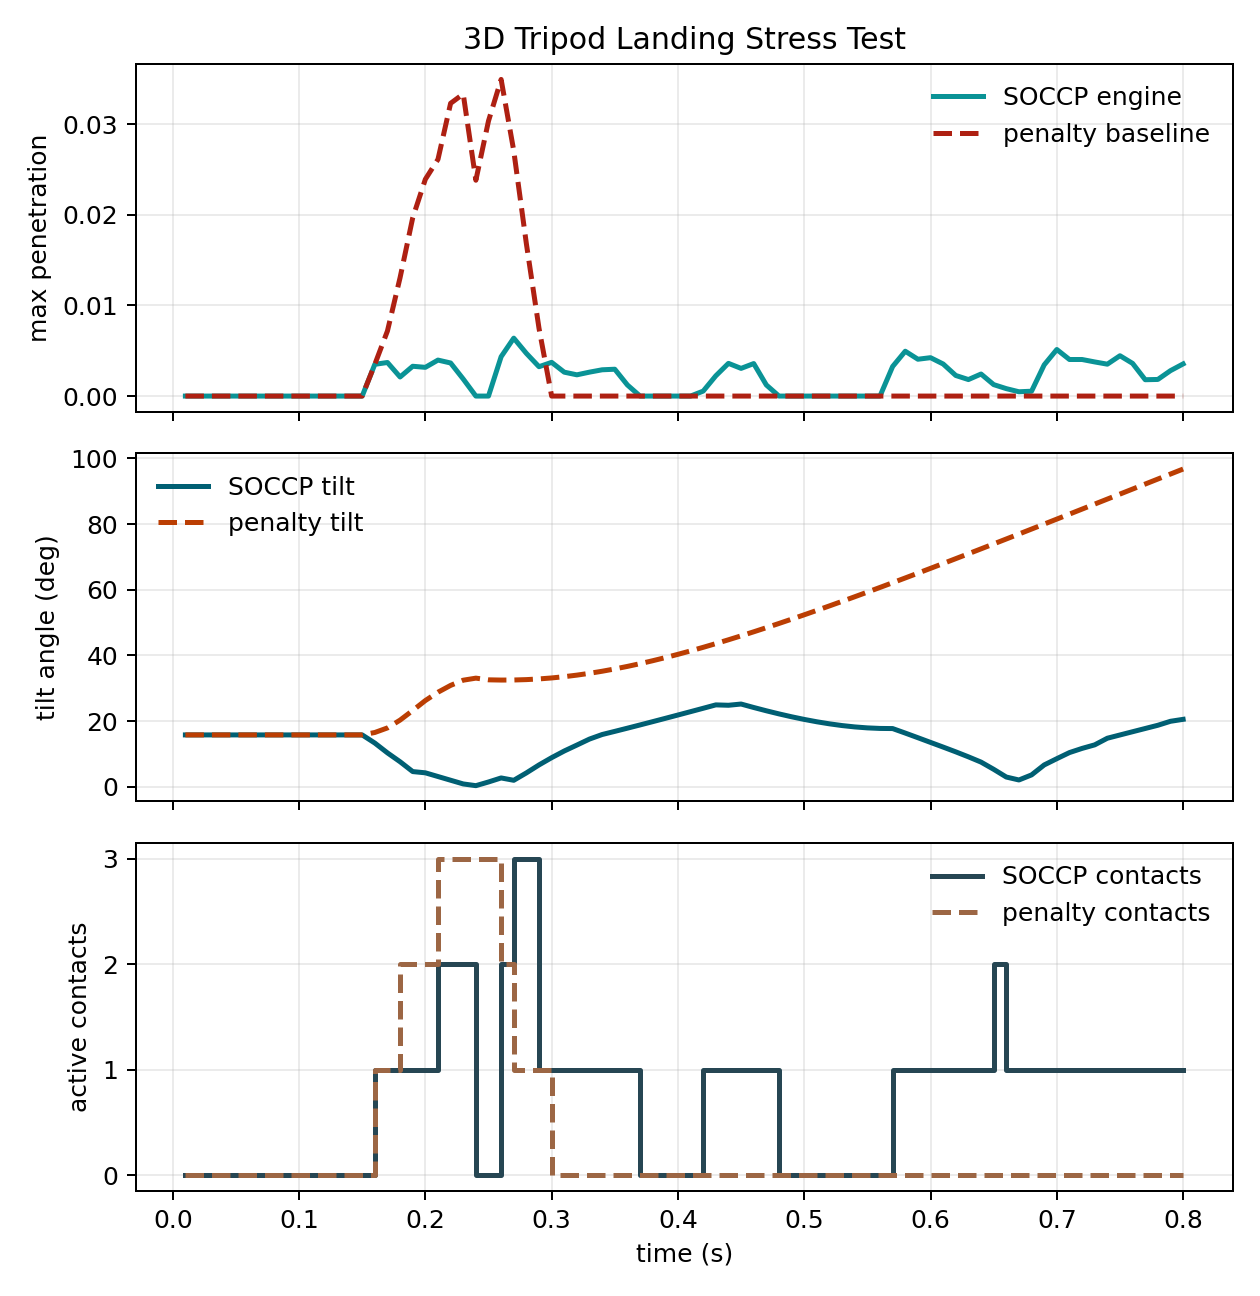
\includegraphics[width=0.78\linewidth]{../../results/benchmark_engine_tripod_landing.png}
    \caption{3D tripod landing stress test 中，SOCCP、full normal LCP与透明调参罚函数三条路径的最大穿透、顶层物体高度、姿态倾角、原始残差以及同时接触数对比。该图既提供normal-only极限下的LCP正确性参照，也展示固定$\Delta t$协议下与tuned penalty之间的取舍。}
    \label{fig:tripod_landing}
\end{figure}

\subsection{补充 solver cross-check：非轴对称3D torsion-free friction中的SOCCP与polyhedral外部基线对照}
\textbf{设置：} 为把 torsion-free friction 主链从``解析滑移+简单PGS''继续推进到``复杂3D场景中的外部交叉验证''，本文新增一个与 oblique-box 同类但显式关闭扭转载荷的非轴对称3D场景：一块带$17^\circ$ yaw 姿态的长方体以预压入状态放置在平面上，初始具有沿$x$和$z$方向的对角滑移速度，但初始法向自旋设为零。该设置保留了非轴对称接触斑、姿态耦合与双切向滑移，同时排除了4D扭转载荷，使问题可以在同一几何族下分别交给去扭转项后的SOCCP三维分支和一个独立 polyhedral-cone 外部基线求解器处理。图\ref{fig:scene_sanity_oblique_polyhedral}给出了该补充对照场景：它不是用来展示4D增量，而是专门检验 torsion-free 3D friction 主链在非平凡3D场景下是否仍与独立锥近似求解器一致。

\begin{figure}[htbp]
    \centering
    \includegraphics[width=0.74\linewidth]{./figures/scene_sanity_oblique_polyhedral.png}
    \caption{非轴对称3D torsion-free friction外部交叉验证场景：带初始yaw姿态的长方体以对角滑移方式在平面上运动，显式关闭法向自旋与扭转载荷，用于比较SOCCP三维分支与独立polyhedral-cone外部基线。}
    \label{fig:scene_sanity_oblique_polyhedral}
\end{figure}

\textbf{结果：} 在这一非平凡3D torsion-free场景中，SOCCP三维分支与 polyhedral 外部基线的峰值等效穿透量分别为$7.0859771\times10^{-3}$与$7.0859677\times10^{-3}$，峰值scaled residual分别为$2.0\times10^{-10}$与$4.0\times10^{-10}$，峰值complementarity violation也分别仅为$2.0\times10^{-10}$与$4.0\times10^{-10}$。更直接的宏观对照量上，两条路径的最大slip差仅为$1.84\times10^{-9}$m，最大spin差为$4.74\times10^{-7}$rad/s，最大倾角差为$1.48\times10^{-6}$rad；末态自旋、末态滑移和末态倾角也都重合到数值精度。也就是说，本文的 torsion-free 3D friction 主链现在已经不再只依赖``解析库仑滑移+friction PGS''这一级证据，而是在一个真正的非轴对称3D场景中继续贴合独立 polyhedral-cone 外部基线。因此，下一小节中的4D/3D/tuned-penalty图可以更干净地解释为``扭转载荷增量改变了什么''，而不是``三维摩擦是否已被验证''。

\begin{figure}[htbp]
    \centering
    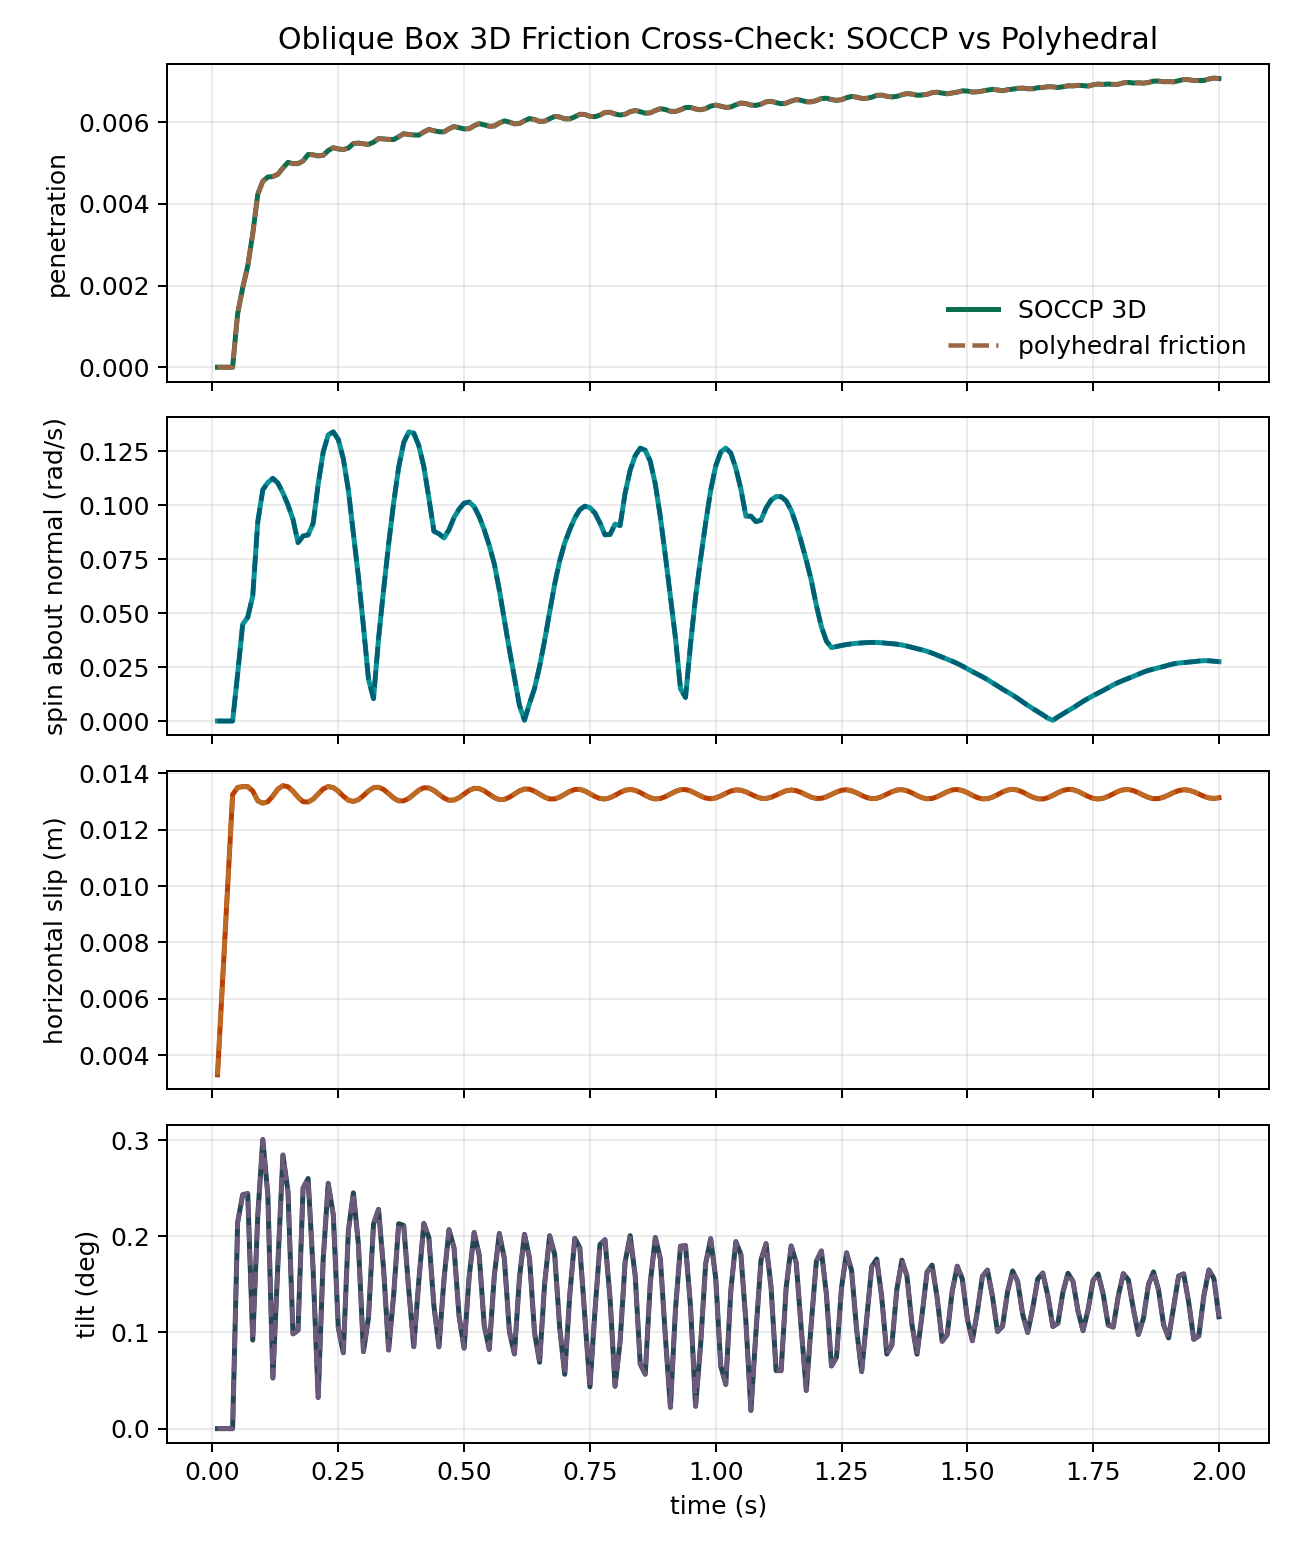
\includegraphics[width=0.80\linewidth]{../../results/benchmark_engine_oblique_box_polyhedral_compare.png}
    \caption{非轴对称3D torsion-free friction外部交叉验证中，SOCCP三维分支与独立polyhedral-cone外部基线在滑移、自旋、姿态、穿透和scaled residual上的对比。两条路径在该非平凡3D场景中几乎重合。}
    \label{fig:oblique_polyhedral_crosscheck}
\end{figure}

\subsection{算例七：非轴对称oblique-box场景中的4D/3D/tuned-penalty三路对比}
\textbf{设置：} 为直接回应``四维摩擦/扭转载荷是否只在轴对称圆柱自旋中有效''这一质疑，本文新增一个更强的3D frictional benchmark：一块带$17^\circ$ yaw 初始姿态的长方体以预压入状态落在平面上，初始时同时具有水平滑移速度与绕接触法线的自旋，从而在有限接触斑上同时激活切向滑移、姿态耦合与扭转载荷。比较三条路径：启用扭转载荷的4D friction、强制$\lambda_\tau=0$的3D torsion-free基线，以及在相同固定时间步协议下透明调参得到的罚函数基线。需要强调的是：\textbf{上一小节已经在相同几何族的非轴对称3D torsion-free 场景中，将SOCCP三维分支与独立polyhedral-cone外部基线做了直接交叉验证。因而本算例的角色被严格收窄为``4D相对3D增加了什么''的动力学消融图，而不是单独的三维摩擦正确性证明图。} 图\ref{fig:scene_case7_oblique_box}给出了该非轴对称oblique-box场景。

\begin{figure}[htbp]
    \centering
    \includegraphics[width=0.76\linewidth]{./figures/scene_case7_oblique_box.png}
    \caption{算例七的模型场景：一个带初始yaw姿态、水平滑移速度和法向自旋的长方体在平面上运动，用于比较4D friction、3D torsion-free基线与透明调参罚函数。}
    \label{fig:scene_case7_oblique_box}
\end{figure}

\textbf{结果：} 该算例中，4D friction、3D torsion-free基线和 tuned penalty 的末态自旋分别为$7.84\times10^{-3}$、$2.61$和$7.27$rad/s；对应末态水平滑移分别为$0.015$、$0.019$和$0.047$m。也就是说，四维摩擦在该非轴对称3D全引擎场景中确实显著改变了宏观动力学：它几乎完全耗散掉法向自旋，并把末态滑移控制在三条路径中的最小值。然而，这个结论并不意味着4D路径在所有指标上都最好。就峰值穿透量而言，4D、3D与tuned penalty分别为$4.54\times10^{-2}$、$3.83\times10^{-2}$和$1.04\times10^{-2}$；就求解器统计而言，4D分支的峰值原始残差为$2.78\times10^{-1}$、并在整个时域中有$1$步触及$180$次迭代上限，而3D基线的峰值残差仅为$8.2\times10^{-9}$、单步最多$30$次迭代。因此，图\ref{fig:engine_oblique_box_friction}的准确用途应是：\textbf{作为4D与3D摩擦结构差异的动力学消融图，说明扭转载荷会改变非轴对称3D场景中的宏观响应；它不应用来单独证明4D分支的正确性。}

\begin{figure}[htbp]
    \centering
    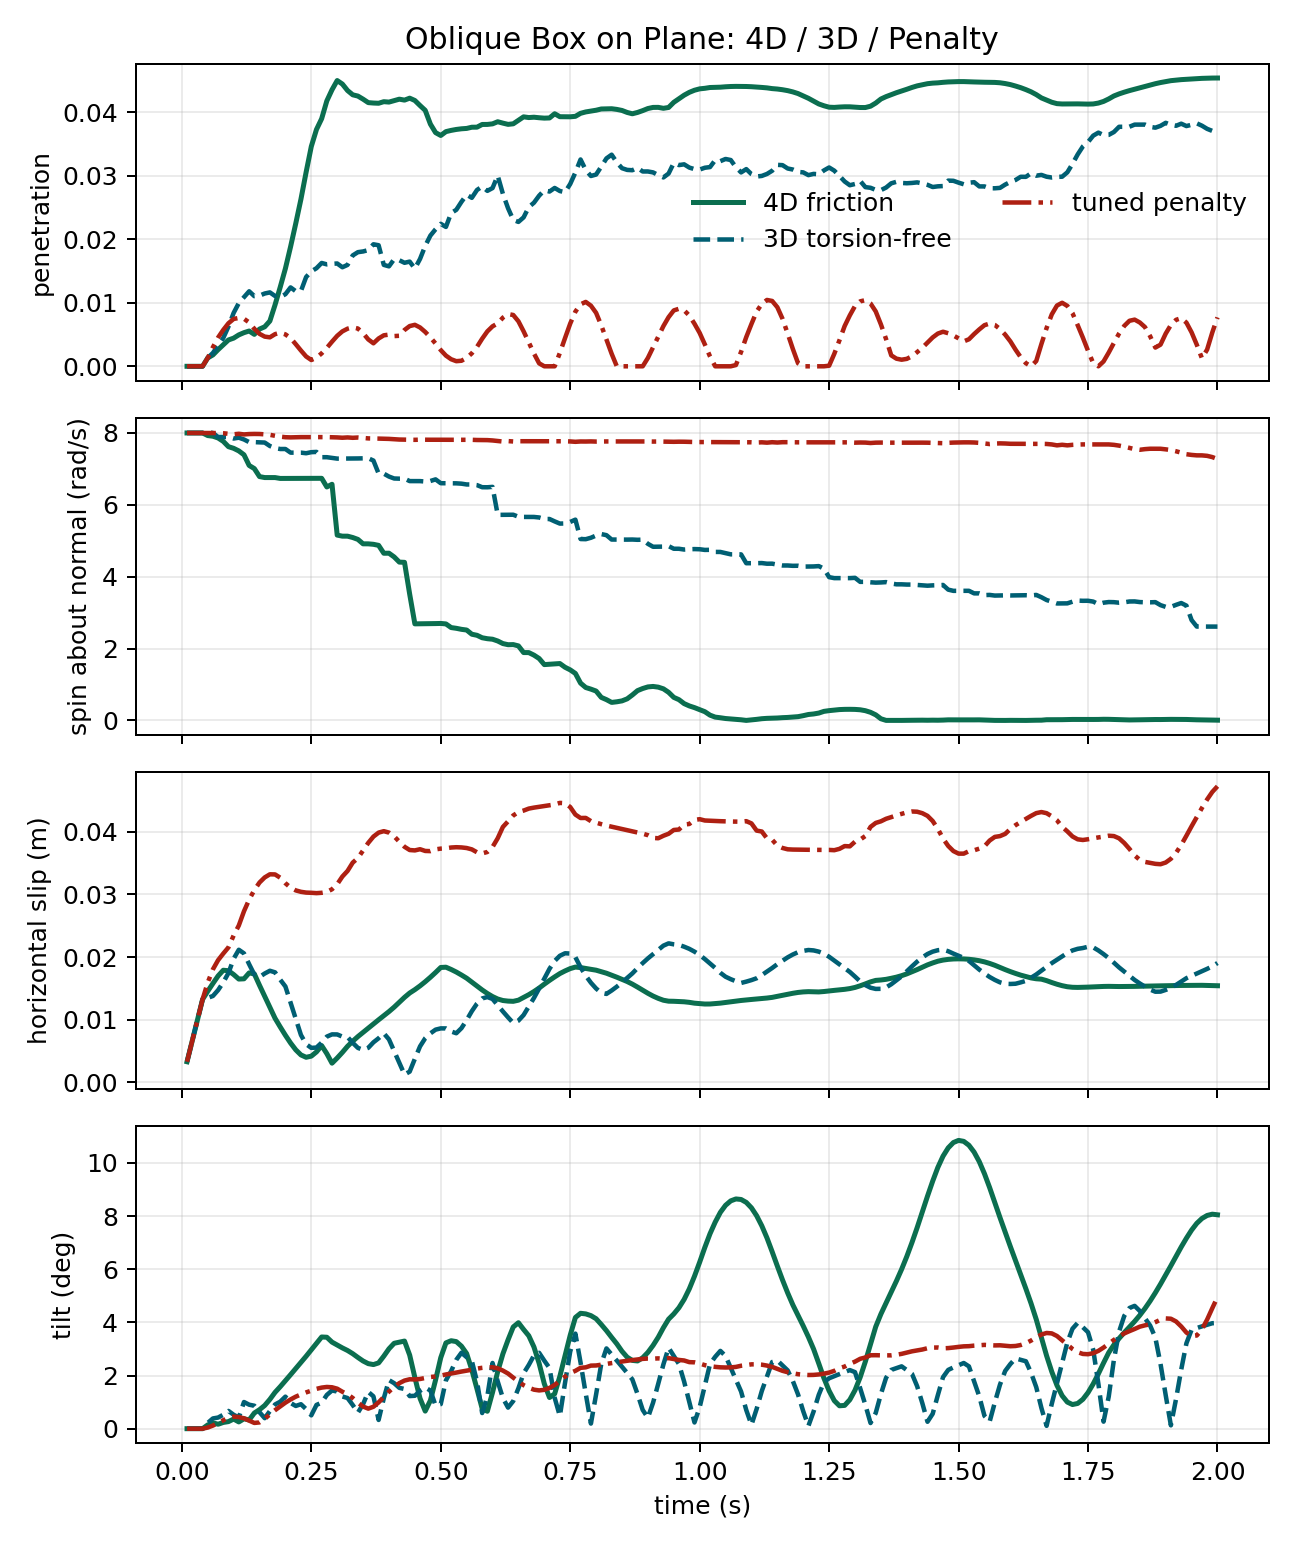
\includegraphics[width=0.80\linewidth]{../../results/benchmark_engine_oblique_box_friction.png}
    \caption{非轴对称oblique-box场景中的动力学消融图：4D friction、3D torsion-free与透明调参罚函数三条路径的穿透、自旋、滑移和姿态对比。该图用于展示四维扭转载荷会改变宏观响应，而非用作单独的正确性证明。}
    \label{fig:engine_oblique_box_friction}
\end{figure}

\subsection{补充验证：两接触盒体堆叠中的解析盒体SDF与闭合三角网格mesh-box SDF对照}
\textbf{设置：} 为进一步回应``当前实验对象是否仍主要局限于解析刚体SDF primitive''这一质疑，本文将原先的单球--支撑体对照升级为一个\textbf{真正的两接触时域场景}：保持与算例四相同的上盒体--下盒体--地面堆叠，只在几何表示层做替换。一条路径中，上下两个动态盒体都采用解析盒体SDF；另一条路径中，上下两个动态盒体都采用由闭合三角网格构造的mesh-box SDF，而地面仍保留解析半空间SDF。这样设置的目的，是把mesh-SDF证据从``单接触支撑面 sanity-check''提升为``多接触时域场景中的解析/mesh 一致性对照''。图\ref{fig:scene_case8_mesh_stack}给出了该两接触盒体堆叠场景。

\begin{figure}[htbp]
    \centering
    \includegraphics[width=0.66\linewidth]{./figures/scene_case4_multicontact_stack.png}
    \caption{两接触盒体堆叠中的解析盒体SDF与闭合三角网格mesh-box SDF对照场景：上下两个动态盒体分别采用解析盒体SDF或mesh-box SDF，地面保持解析半空间SDF。}
    \label{fig:scene_case8_mesh_stack}
\end{figure}

\textbf{结果：} 在这一两接触时域对照中，解析盒体SDF与mesh-box SDF两条路径的上层盒体质心高度差、竖直速度差和峰值穿透差分别仅为$1.33\times10^{-9}$、$2.29\times10^{-8}$和$1.20\times10^{-10}$；两者的峰值穿透都为$2.963\times10^{-2}$m，接触数轨迹也完全一致。求解器统计方面，二者的峰值scaled residual都为$7.14\times10^{-8}$，峰值锥互补违约都为$5.2\times10^{-9}$。也就是说，在这个真正的两接触时域场景中，当前主链已经不再局限于解析 primitive，而能够在不改动力学、求解器或积分策略的前提下直接接受闭合三角网格导出的mesh-SDF，并保持与解析盒体SDF几乎完全一致的宏观运动和数值诊断。需要强调的是，这仍只说明本文已经跨出了``纯解析体''的实验口径，而不应被夸大为对任意复杂网格SDF、噪声几何或工业规模三角网格的全面验证。

\begin{figure}[htbp]
    \centering
    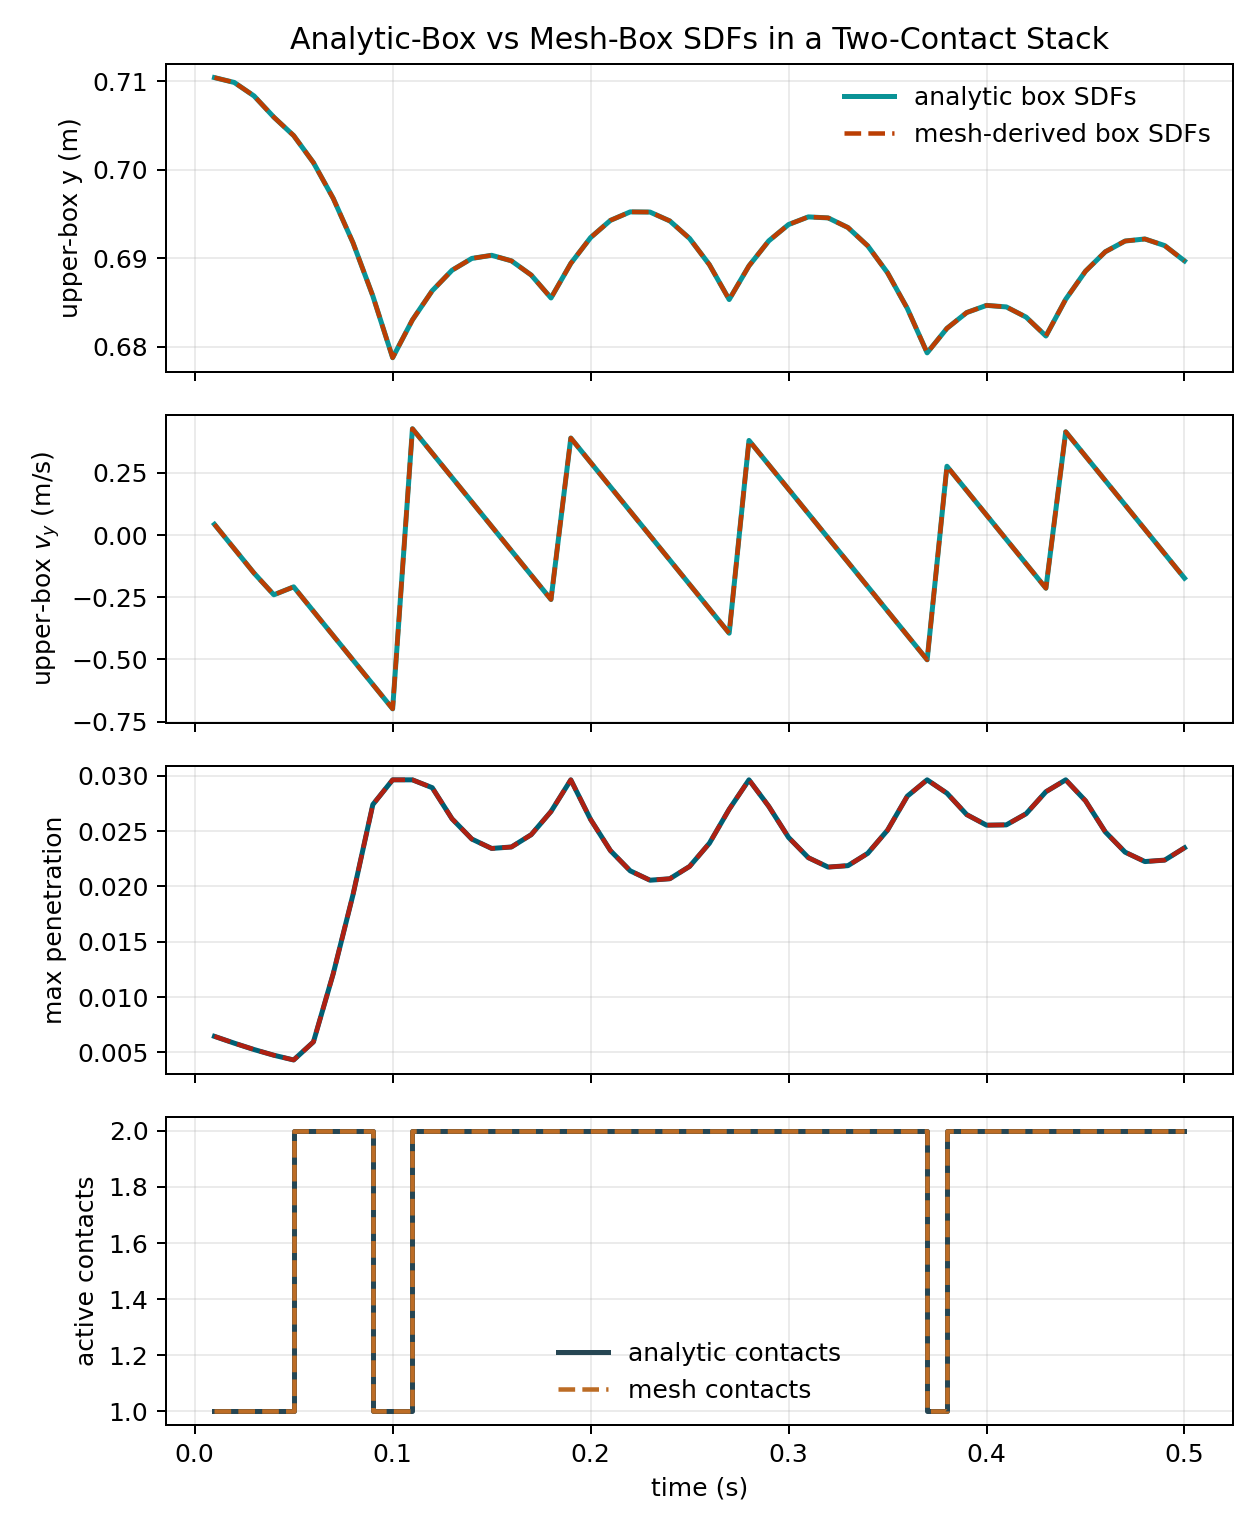
\includegraphics[width=0.78\linewidth]{../../results/benchmark_engine_mesh_sdf_multicontact.png}
    \caption{两接触盒体堆叠中的解析盒体SDF与闭合三角网格mesh-box SDF对照：上层盒体高度、竖直速度、峰值穿透和接触数的时间历程在两条路径上几乎重合。}
    \label{fig:engine_mesh_sdf_multicontact}
\end{figure}

\subsection{补充收敛统计与口径说明}
为避免把``宏观运动稳定''与``数值残差已充分收敛''混为一谈，表\ref{tab:solver_convergence}统一报告本文几个关键时域算例中的\textbf{原始残差无穷范数}、95分位原始残差、\textbf{scaled residual}、\textbf{complementarity violation}、最大单步迭代数以及触及迭代上限的步数。这里的scaled residual均由各求解器按速度/冲量/锥变量的当前尺度做无量纲归一化；complementarity violation则统一取与各求解器自身正交锥或二阶锥互补结构一致的无量纲违约，\textbf{不再使用未经归一化的$\lambda_n u_n$乘积作为跨算例口径}。因此，表中raw residual主要用于比较同一实现链内部的数值难度，而scaled residual与complementarity violation则更适合做不同状态规模下的统一收敛判定。本文凡称``收敛''，均指对应求解器在给定步内达到所设残差阈值；若某条路径只是给出可重复的宏观结果，但峰值原始残差仍偏高，则正文明确将其表述为``原型级可运行证据''而非``强收敛性证明''。

\begin{table}[htbp]
    \centering
    \caption{关键时域算例的统一残差、互补违约与迭代统计}
    \label{tab:solver_convergence}
    \scriptsize
    \setlength{\tabcolsep}{4pt}
    \renewcommand{\arraystretch}{1.15}
    \resizebox{\linewidth}{!}{
    \begin{tabular}{p{3.3cm}p{1.4cm}p{2.0cm}p{2.0cm}p{2.0cm}p{2.0cm}p{1.7cm}p{1.9cm}}
        \toprule
        场景 & 分支 & 峰值raw residual & 95分位raw residual & 峰值scaled residual & 峰值complementarity violation & 最大迭代数 & 达到迭代上限步数 \\
        \midrule
        圆柱自旋对比 & 4D & $3.05\times10^{0}$ & $3.03\times10^{0}$ & $1.13\times10^{-4}$ & $6.21\times10^{-8}$ & $12$ & $0$ \\
        圆柱自旋对比 & 3D & $8.99\times10^{-1}$ & $7.63\times10^{-9}$ & $1.49\times10^{-3}$ & $1.91\times10^{-3}$ & $32$ & $0$ \\
        耦合4D参考 & SOCCP & $0$ & $0$ & $0$ & $0$ & $11$ & $0$ \\
        耦合4D参考 & FourDPGS & $0$ & $0$ & $0$ & $0$ & $2$ & $0$ \\
        两接触normal-only & SOCCP & $2.89\times10^{-1}$ & $2.83\times10^{-1}$ & $7.14\times10^{-8}$ & $5.20\times10^{-9}$ & $17$ & $0$ \\
        两接触normal-only & NormalLCP & $2.89\times10^{-1}$ & $2.83\times10^{-1}$ & $2.89\times10^{-1}$ & $2.89\times10^{-1}$ & $160$ & $40$ \\
        tripod normal-only & SOCCP & $1.22\times10^{-2}$ & $6.32\times10^{-9}$ & $1.12\times10^{-8}$ & $6.90\times10^{-9}$ & $17$ & $0$ \\
        tripod normal-only & NormalLCP & $5.78\times10^{-3}$ & $4.91\times10^{-9}$ & $2.63\times10^{-3}$ & $2.63\times10^{-3}$ & $180$ & $3$ \\
        oblique-box friction & 4D & $2.78\times10^{-1}$ & $6.28\times10^{-9}$ & $4.12\times10^{-2}$ & $8.90\times10^{-4}$ & $180$ & $1$ \\
        oblique-box friction & 3D & $8.20\times10^{-9}$ & $2.80\times10^{-9}$ & $1.10\times10^{-9}$ & $6.90\times10^{-9}$ & $30$ & $0$ \\
        oblique-box polyhedral & SOCCP-3D & $9.40\times10^{-9}$ & $6.91\times10^{-9}$ & $2.00\times10^{-10}$ & $2.00\times10^{-10}$ & $11$ & $0$ \\
        oblique-box polyhedral & Polyhedral & $9.90\times10^{-9}$ & $9.70\times10^{-9}$ & $4.00\times10^{-10}$ & $4.00\times10^{-10}$ & $75$ & $0$ \\
        质量比扫描 & SOCCP & $0$ & $0$ & $0$ & $0$ & $6$ & $0$ \\
        \bottomrule
    \end{tabular}
    }
\end{table}

\section{结论}
本文建立了一套系统、严密的基于SDF的体积接触动力学框架。本文的核心理论创新在于：以局部重叠深度的矩比泛函构造量纲一致的形状感知等效间隙；以统一权函数测度定义等效接触中心、法线与扭转惯性半径；并通过退化正则化的四维摩擦锥将有限接触斑摩擦与经典点接触库仑摩擦统一在同一理论框架内。结合SOCCP与Fischer--Burmeister半光滑牛顿求解，本文进一步把上述理论链条落成了一条可运行的原型级数值实现。

从证据链角度看，本文现在已经具备六类互补支撑。第一类是\textbf{解析或经典参照验证}：圆柱算例中代码计算的等效扭转半径与经典有效力臂误差为$4.00\%$，对应停止时间误差为$3.85\%$；受控扭转载荷 sanity-check 中，SOCCP四维分支对解析阻转曲线的最大角速度误差小于$10^{-13}$、停转时间误差为$4.37\%$；单球自由落体 sanity-check 中，SOCCP与full normal LCP在碰撞前严格贴合解析自由落体轨迹，在接触阶段又重合到数值精度；平动主导滑移摩擦 sanity-check 中，SOCCP三维分支、独立 friction PGS 与独立 polyhedral friction 外部基线又共同复现了解析库仑滑移曲线，停止时间均为$0.250$s，停止距离均为$0.12692$m。第二类是\textbf{独立求解器交叉验证}：在固定接触斑且同时激活$v_x$、$v_z$与$\omega_y$的耦合4D参考中，SOCCP与独立4D PGS都给出零scaled residual、零锥互补违约和相同的末态自旋，而累计滑移差与yaw角差分别仅为$1.57\times10^{-2}$m与$1.68\times10^{-2}$rad，这说明4D响应并非某一SOCCP实现特有的数值产物。第三类是\textbf{非轴对称3D外部摩擦基线验证}：在新增的torsion-free oblique-box对照中，SOCCP三维分支与独立polyhedral-cone外部基线的最大slip/spin差仅为$1.80\times10^{-9}$m与$4.74\times10^{-7}$rad/s，最大倾角差也仅为$1.48\times10^{-6}$rad，且两条路径的峰值scaled residual都在$10^{-10}$量级，这说明本文的三维摩擦主链已经不再只依赖解析滑移和简单PGS，而是在一个非平凡3D场景中继续贴合独立外部基线。第四类是\textbf{理论退化与局部鲁棒性验证}：对称两接触normal-only算例中，SOCCP、引擎级法向LCP与罚函数三条分支给出了相同的峰值穿透量$2.963\times10^{-2}$；而在更强的tripod normal-only算例中，SOCCP与full normal LCP又进一步在峰值穿透上重合到$6.392\times10^{-3}$量级，从而为图\ref{fig:tripod_landing}重新提供了LCP正确性参照；受控二接触质量比扫描算例中，质量比从$1$提高到$1000$时，SOCCP/半光滑牛顿求解器始终在$6$步内收敛。第五类是\textbf{比较性动力学证据}：全引擎圆柱自旋对比表明，四维摩擦锥在$1.2$s时将残余角速度降至$1.58\times10^{-5}$rad/s，而去掉扭转项的三维基线仍保留$2.19$rad/s；非轴对称oblique-box场景进一步表明，4D friction 可将末态自旋压到$7.84\times10^{-3}$rad/s，并把末态滑移控制到$0.015$m，而3D torsion-free与tuned penalty分别保留更高的残余自旋或更大的滑移，但该图仅应理解为动力学消融而非正确性证明。第六类是\textbf{几何外延性验证}：在两接触盒体堆叠场景中，解析盒体SDF与闭合三角网格mesh-box SDF两条路径的上层盒体高度、竖直速度与峰值穿透差分别仅为$1.33\times10^{-9}$、$2.29\times10^{-8}$和$1.20\times10^{-10}$，而峰值scaled residual与锥互补违约也都维持在$10^{-8}$到$10^{-9}$量级，从而说明本文主链已经跨出``只能处理解析primitive''的最窄实验口径。

这些结果支持的最准确结论是：本文提出的几何压缩、四维摩擦结构与SOCCP主链已经具备明确的可计算意义。对于退化链路，normal-only 主链已经由自由落体与LCP对照验证，torsion-free friction 主链也已经由解析库仑滑移、friction PGS 与非轴对称3D polyhedral-cone外部基线补成了多层 correctness / cross-check 证据；对于四维扭转载荷本身，受控扭转参考已经把``4D锥+求解器''补成了独立的正确性证据，新的耦合4D solver cross-check又进一步说明这一响应能够被独立4D projected solver重复得到，而轴对称与非轴对称两个全引擎场景则继续说明扭转载荷会改变完整动力学；对于几何外延性，两接触盒体堆叠中的解析/mesh-box 对照又表明当前主链已能接受一个最小但真实的mesh-derived SDF输入，并在多接触时域场景中保持一致。与此同时，本文现在已经统一导出了raw residual、scaled residual与formulation-consistent complementarity violation，使关键时域算例的收敛口径不再停留在单一raw residual层面。但本文同样明确保留了当前实现的边界。其一，均匀体素原型仅对$p=2\sim4$给出可防守的工程性主张，其中$p=2$为默认稳健配置、$p=4$为较细网格下的增强选项，而$p=6$仅用于展示理论聚焦趋势。其二，透明调参后的tripod fair-baseline 比较表明，SOCCP与NormalLCP在normal-only物理模型下彼此一致，但二者相对tuned penalty并不在所有姿态指标上系统性占优。其三，oblique-box friction 算例表明当前4D分支也是数值上最困难的一条路径，因此该图只能作为动力学消融证据，而不是独立的正确性证明。其四，本文虽然已把mesh-SDF证据升级到两接触盒体堆叠，但这仍不足以外推到任意复杂网格SDF、噪声几何、柔性体或工业规模多接触系统。

因此，本文更适合被定位为：\textbf{一篇完成了理论闭环、原型实现和初步比较验证的方法论文}，而不是一篇已经穷尽复杂工程场景比较的最终工程论文。后续工作将优先集中于四件事：引入自适应八叉树积分以支撑更高$p$；补充带扭转载荷的外部基线、polyhedral MLCP/LCP的更严格实现以及更强文献级比较；改进接触激活阶段的全局化策略；并在更复杂的mesh-SDF、噪声几何与柔性体耦合问题上继续扩展当前框架。

\appendix

\section{等效间隙与深度矩的附录证明}

\begin{lemma}[矩比的概率测度表示]\label{lem:prob_measure}
若$I_{p-1}(\bm{q}) > 0$，则$w_p(\bm{x};\bm{q}) dV$是$\Omega(\bm{q})$上的概率测度，且
\begin{equation}
    -g_{eq}^{(p)}(\bm{q}) = \int_{\Omega(\bm{q})} \delta(\bm{x};\bm{q}) w_p(\bm{x};\bm{q}) dV .
\end{equation}
\end{lemma}

\begin{proof}
由式(\ref{eq:wp})可得$w_p \ge 0$且$\int_{\Omega(\bm{q})} w_p dV = 1$，故$w_p dV$为概率测度。再将式(\ref{eq:wp})代入上式右端，有
\begin{equation}
    \int_{\Omega(\bm{q})} \delta w_p dV = \frac{1}{I_{p-1}(\bm{q})} \int_{\Omega(\bm{q})} \delta^p dV = \frac{I_p(\bm{q})}{I_{p-1}(\bm{q})} = -g_{eq}^{(p)}(\bm{q}).
\end{equation}
即得结论。
\end{proof}

\begin{lemma}[深度矩的对数凸性]\label{lem:logconvex}
对任意$r > 1$，深度矩满足
\begin{equation}
    I_r(\bm{q})^2 \le I_{r-1}(\bm{q}) I_{r+1}(\bm{q}).
\end{equation}
\end{lemma}

\begin{proof}
将$I_r$写为$ I_r = \int_{\Omega(\bm{q})} \delta^{\frac{r-1}{2}} \delta^{\frac{r+1}{2}} dV$，对上式应用Cauchy--Schwarz不等式，便得到所述结论。因此$\log I_r$关于$r$是凸的。
\end{proof}

\begin{proof}[命题\ref{prop:basic}的证明]
由$[\delta] = L$和$[dV] = L^3$立刻得到$[I_r] = L^{r+3}$，因此$ \left[ \frac{I_p}{I_{p-1}} \right] = L $，从而$g_{eq}^{(p)}$具有长度量纲。其次，$\delta \ge 0$蕴含$I_p \ge 0$与$I_{p-1} \ge 0$，故由定义\ref{def:geq}有$g_{eq}^{(p)} \le 0$。当$I_{p-1} = 0$时，$\delta^{p-1} = 0$几乎处处成立，于是$\delta = 0$几乎处处成立；反之若存在正测度子集使$\delta > 0$，则$I_{p-1} > 0$。最后，由引理\ref{lem:prob_measure}，$-g_{eq}^{(p)}$是$\delta$在概率测度$w_p dV$下的均值，因此有$ 0 \le -g_{eq}^{(p)} \le \delta_{\max}$。命题得证。
\end{proof}

\begin{proof}[命题\ref{prop:monotone}的证明]
由引理\ref{lem:logconvex}，对任意$r > 1$有$I_r^2 \le I_{r-1} I_{r+1}$。将其改写为$ \frac{I_r}{I_{r-1}} \le \frac{I_{r+1}}{I_r} $，即可得相邻矩比关于$r$单调不减。令$r = p-1$，便有$ -g_{eq}^{(p)} = \frac{I_p}{I_{p-1}} $关于$p$单调不减。再结合命题\ref{prop:basic}给出的上界$\delta_{\max}$，可知该序列单调有界，因此极限存在。另一方面，对任意$\varepsilon > 0$，集合$\{ \delta > \delta_{\max} - \varepsilon \}$具有正测度，故当$p \to \infty$时，高阶矩由该集合主导，从而$ \lim_{p \to \infty} \frac{I_p}{I_{p-1}} = \delta_{\max} $。因此结论成立。
\end{proof}

\begin{proof}[定理\ref{thm:sharp}的证明]
由定理假设，对任意凸增函数$\varphi$均有$ \int \varphi(\delta_1) dV \ge \int \varphi(\delta_2) dV $。特别地，对$r \ge 1$取$\varphi_r(t) = t^r$，得到$I_r[\delta_1] \ge I_r[\delta_2]$。记$M_i(r) = \log I_r[\delta_i]$。由引理\ref{lem:logconvex}知$M_i(r)$关于$r$为凸函数；而majorization假设意味着峰化程度更强的$\delta_1$在高阶矩上增长更快，因此差函数$M_1(r) - M_2(r)$在$r \ge 1$上单调不减。于是于$r = p-1$有$ M_1(p) - M_1(p-1) \ge M_2(p) - M_2(p-1) $。两侧取指数即得$ \frac{I_p[\delta_1]}{I_{p-1}[\delta_1]} \ge \frac{I_p[\delta_2]}{I_{p-1}[\delta_2]} $，亦即$ -g_{eq}^{(p)}[\delta_1] \ge -g_{eq}^{(p)}[\delta_2] $。定理得证。
\end{proof}

\section{方向导数与小穿透极限的附录证明}

\begin{proof}[定理\ref{thm:jac}的证明]
取固定有界盒$D \subset \mathbb{R}^3$，使所有考虑的接触斑都包含于$D$中，并定义零延拓函数$ \bar{\delta}(\bm{x};\bm{q}) = \delta(\bm{x};\bm{q}) \chi_{\Omega(\bm{q})}(\bm{x}) $。于是$I_r(\bm{q}) = \int_D \bar{\delta}(\bm{x};\bm{q})^r dV$。令$\bm{q}_{\varepsilon} = \bm{q} + \varepsilon \, \delta \bm{q}$，则有
\begin{equation}
    \frac{I_r(\bm{q}_{\varepsilon}) - I_r(\bm{q})}{\varepsilon} = \int_D \frac{\bar{\delta}(\bm{x};\bm{q}_{\varepsilon})^r - \bar{\delta}(\bm{x};\bm{q})^r}{\varepsilon} dV.
\end{equation}
由于$\phi_A$和$\phi_B$在假设\ref{ass:sdf}下全局Lipschitz且分片$C^1$，$\bar{\delta}$对$\bm{q}$的方向导数几乎处处存在，并且可由可积函数主导。由均值定理和主导收敛定理，可将极限移入积分号内，得到$ D I_r(\bm{q})[\delta \bm{q}] = r \int_D \bar{\delta}^{r-1} D\bar{\delta}[\delta \bm{q}] dV $。又因为$\bar{\delta} = 0$在$\partial \Omega(\bm{q})$上成立，移动边界带来的运输项乘零而消失，故上式可缩回到$\Omega(\bm{q})$上，得到正文中的方向导数公式。对于$\delta = \min\{\delta_A,\delta_B\}$的不可导集合$\mathcal{S}(\bm{q})$，由假设\ref{ass:domain}，该集合要么零测，要么可由Clarke广义导数处理，因此不影响上述结论。最后对矩比$g_{eq}^{(p)} = -I_p/I_{p-1}$应用商法则，并代入$ D \delta = \nabla \delta^T \bm{J}_{kin} \, \delta \bm{q} $，便得到式(\ref{eq:jac_general})与式(\ref{eq:Jn_new})。定理得证。
\end{proof}

\begin{proof}[定理\ref{thm:consistency}的证明]
在假设\ref{ass:small}下，于接触点邻域作变量代换$ \bm{x} = \bm{x}_c + \ell(\bm{q}) \bm{\xi} $。由$\delta(\bm{x};\bm{q}) = \delta_n(\bm{q}) \hat{\delta}(\bm{\xi}) + o(\delta_n)$和$dV = \ell^3 d\bm{\xi}$，可得对任意$r > 0$有$ I_r(\bm{q}) = \delta_n(\bm{q})^r \ell(\bm{q})^3 \hat{I}_r + o\!\left( \delta_n^r \ell^3 \right) $。对$r = p$与$r = p-1$分别应用上式，得到$ \frac{I_p}{I_{p-1}} = \delta_n \frac{\hat{I}_p}{\hat{I}_{p-1}} + o(\delta_n) = c_p \delta_n + o(\delta_n) $，故$ g_{eq}^{(p)}(\bm{q}) = -c_p \delta_n(\bm{q}) + o(\delta_n) $。再看接触中心，由$w_p$的定义与同样的变量代换，可得$ \bm{p}_c - \bm{x}_c = \ell \frac{\int \bm{\xi} \, \hat{\delta}(\bm{\xi})^{p-1} d\bm{\xi}}{\hat{I}_{p-1}} + o(\ell) $，因此$\bm{p}_c \to \bm{x}_c$。对于法线，由SDF正则性与小接触斑假设，$\nabla \delta(\bm{x};\bm{q})$在接触点邻域可写为$\bm{n}_{clas} + o(1)$，于是$ \bm{n}^* = \int_{\Omega(\bm{q})} \nabla \delta \, w_p dV = \bm{n}_{clas} + o(1) $，归一化后即得$\bm{n}_c \to \bm{n}_{clas}$。定理成立。
\end{proof}

\section{几何压缩、摩擦退化与SOCCP合理性的附录证明}

\begin{proof}[命题\ref{prop:rigid}的证明]
对叠加刚体运动$\bm{x}' = \bm{R}\bm{x} + \bm{c}$作变量替换。由于$\bm{R} \in SO(3)$，有$\det \bm{R} = 1$，故体积测度保持不变；同时向量长度、内积与叉乘范数在旋转下不变，因此$\delta$、$I_r$与$g_{eq}^{(p)}$保持不变。对接触中心，有$ \bm{p}_c' = \int (\bm{R}\bm{x} + \bm{c}) w_p dV = \bm{R}\bm{p}_c + \bm{c} $。法线满足$\bm{n}^{*\prime} = \bm{R}\bm{n}^*$，归一化后得$\bm{n}_c' = \bm{R}\bm{n}_c$；扭转惯性半径由式(\ref{eq:rtau})以及叉乘范数的不变性可知也保持不变。故命题成立。
\end{proof}

\begin{proof}[命题\ref{prop:variance}的证明]
对任意固定广义速度$\bm{v}$，记$ \bm{F}(\bm{x}) = \bm{B}(\bm{x}) \bm{v} $，$ \bar{\bm{F}} = \int_{\Omega(\bm{q})} \bm{F}(\bm{x}) w_p dV = \bm{J}_t \bm{v} $。于是$\bm{F}(\bm{x}) = \bar{\bm{F}} + (\bm{F}(\bm{x}) - \bar{\bm{F}})$。两侧取欧氏范数平方并对$\Omega(\bm{q})$积分，得到式(\ref{eq:variance})；其中交叉项为零，因为$\int_{\Omega(\bm{q})} (\bm{F} - \bar{\bm{F}}) w_p dV = 0$。命题得证。
\end{proof}

\begin{proof}[定理\ref{thm:degenerate}的证明]
记接触斑直径满足$\operatorname{diam}(\Omega(\bm{q})) \le C \ell(\bm{q})$。于是对任意$\bm{x} \in \Omega(\bm{q})$有$ \| (\bm{x} - \bm{p}_c) \times \bm{n}_c \| \le \|\bm{x} - \bm{p}_c\| \le C\ell $，故由式(\ref{eq:rtau})可得$r_\tau = O(\ell)$。若$\bm{B}(\bm{x})$在接触点邻域内Lipschitz连续，则$ \| \bm{B}(\bm{x}) - \bm{J}_t \| \le LC\ell $，将其代入式(\ref{eq:variance})即可得涨落项为$O(\ell^2 \|\bm{v}\|^2)$，因此当$\ell \to 0$时趋于零。再看摩擦锥约束。若$\bm{\lambda}_t^{(k)} \in K_{\varepsilon_\tau^{(k)}}(\lambda_n^{(k)})$，则由式(\ref{eq:cone_reg})有$ \left| \frac{\lambda_\tau^{(k)}}{\hat{r}_\tau^{(k)}} \right| \le \mu \lambda_n^{(k)} $，于是$ |\lambda_\tau^{(k)}| \le \mu \lambda_n^{(k)} \hat{r}_\tau^{(k)} $。当$\{\lambda_n^{(k)}\}$有界且$\varepsilon_\tau^{(k)} \to 0$、$r_\tau^{(k)} = O(\ell_k) \to 0$时，有$\hat{r}_\tau^{(k)} \to 0$，故$\lambda_\tau^{(k)} \to 0$。极限中仅剩$ \| (\lambda_{t1},\lambda_{t2})^T \| \le \mu \lambda_n $，即经典三维库仑锥。定理得证。
\end{proof}

\begin{proof}[推论\ref{cor:soccp}的证明]
定理\ref{thm:jac}表明法向约束来自一个具有明确定义方向导数的等效间隙，因此法向互补关系不是凭空指定，而是直接由分布式重叠几何诱导。命题\ref{prop:variance}表明切向雅可比$\bm{J}_t$保留了分布式滑移映射的一阶矩，而其误差项正是可量化的二阶涨落。定理\ref{thm:degenerate}进一步保证当接触斑塌缩时，这一有限维压缩自动退化到经典点接触摩擦理论。将这三条结果合并，便得到正文中的SOCCP并非任意的代数离散，而是分布式接触几何与摩擦耗散经有限维压缩后的结构保持表述。推论得证。
\end{proof}

\begin{thebibliography}{99}

\bibitem{lu2011isogeometric}
J.~Lu.
Isogeometric contact analysis: Geometric basis and formulation for frictionless contact.
\emph{Computer Methods in Applied Mechanics and Engineering}, 200(5--8):726--741, 2011.
doi:10.1016/j.cma.2010.10.001.

\bibitem{noels2006crashworthiness}
L.~Noels, L.~Stainier, and J.-P.~Ponthot.
Simulation of crashworthiness problems with improved contact algorithms for implicit time integration.
\emph{International Journal of Impact Engineering}, 32(5):799--825, 2006.
doi:10.1016/j.ijimpeng.2005.04.010.

\bibitem{hunek1993penalty}
I.~Hunek.
On a penalty formulation for contact-impact problems.
\emph{Computers \& Structures}, 48(2):193--203, 1993.
doi:10.1016/0045-7949(93)90210-X.

\bibitem{kolman2021bipenalty}
R.~Kolman, I.~Necoara, and A.~Manei.
Bi-penalty stabilized technique with predictor-corrector time scheme for contact-impact problems of elastic bars.
\emph{Mathematics and Computers in Simulation}, 184:305--324, 2021.
doi:10.1016/j.matcom.2020.11.014.

\bibitem{leichner2019implicit}
A.~Leichner, H.~Andr"a, and B.~Simeon.
A contact algorithm for voxel-based meshes using an implicit boundary representation.
\emph{Computer Methods in Applied Mechanics and Engineering}, 352:276--299, 2019.
doi:10.1016/j.cma.2019.04.008.

\bibitem{lorez2024eulerian}
F.~Lorez, M.~Pundir, and D.~S.~Kammer.
Eulerian framework for contact between solids represented as phase fields.
\emph{Computer Methods in Applied Mechanics and Engineering}, 418:116497, 2024.
doi:10.1016/j.cma.2023.116497.

\end{thebibliography}

\end{document}
